%------------------------------------------------------------%

\chapter{Resultados}

Este apêndice consolida todos os resultados detalhados levantados durante a execução deste trabalho. Ele serve como um repositório completo dos dados obtidos a partir dos experimentos realizados com os modelos de aprendizado de máquina, os quais foram treinados sobre os diferentes conjuntos de dados gerados e descritos ao longo do texto principal.

Relembrando, os testes foram conduzidos com o objetivo de avaliar o desempenho da abordagem proposta em dois cenários distintos: (i) validação cruzada com os dados do robô principal, englobando tanto simulações quanto coletas reais, e (ii) testes de portabilidade em duas outras topologias robóticas simuladas, utilizados para verificar a robustez dos modelos e do sensor multimodal diante de variações físicas e estruturais.

A organização dos resultados apresentada a seguir mantém a estrutura originalmente planejada: os dados estão agrupados de acordo com a origem (topologia principal [simulado ou real] ou topologias secundárias). Dentro de cada grupo, são apresentados separadamente para cada tipo de \textit{dataset} processado: imagens brutas da câmera de profundidade, dados brutos do \textit{LiDAR}, \textit{features} extraídas das imagens, \textit{features} extraídas do \textit{LiDAR}, e a combinação dessas \textit{features}. Para cada um destes cenários, são exibidas tabelas com as métricas quantitativas de desempenho — acurácia média, perda final, tempo de validação e época final (quando aplicável) — para os cinco modelos de aprendizado de máquina avaliados. Matrizes de confusão também são apresentadas nos casos em que auxiliam na compreensão dos resultados, sobretudo quando o desempenho foi inferior ao esperado ou quando ocorreram confusões significativas entre as classes de interesse.

\section{Resultados com o robô principal}

Nesta seção são apresentados os resultados obtidos com os dados provenientes do robô principal, utilizado tanto em ambiente simulado quanto em testes reais em laboratório. Para ambas as origens, foi aplicada a técnica de validação cruzada, conforme descrito anteriormente. Os resultados estão organizados em subseções separadas, de modo a permitir uma análise clara do desempenho dos modelos em cada tipo de \textit{dataset}. Cada conjunto de dados — imagens brutas, leituras do \textit{LiDAR}, \textit{features} extraídas e combinação de \textit{features} — é avaliado individualmente, permitindo comparar o impacto de diferentes formas de representação dos dados na tarefa de classificação. As métricas consideradas incluem acurácia média, tempo de validação, perda final e número de épocas, além da matriz de confusão quando relevante. A distinção entre os resultados simulados e reais permite também avaliar a consistência dos modelos frente à variação entre os ambientes.

\subsection{Dados simulados}

Nesta subseção são apresentados os resultados obtidos a partir dos dados simulados gerados pelo robô principal durante as execuções no ambiente virtual.

\subsubsection{Imagens brutas}

Para avaliar as imagens foi utilizado a \textit{SqueezeNet}. O \textit{dataset} utilizado nesta etapa contém imagens de profundidade capturadas por simulação no robô principal, organizadas em quatro classes: amortecedor, isolador, sinalizador e nada. O treinamento foi conduzido utilizando validação cruzada com 5 dobras. A Tabela~\ref{tab:squeezenet_camera} apresenta os resultados obtidos, mo final da tabela são mostradas as médias dos resultados.

\begin{table}[H]
\centering
\caption{Desempenho da SqueezeNet com imagens brutas (simulação)}
\label{tab:squeezenet_camera}
\begin{tabular}{ccccc}
\hline
\textbf{Dobra} & \textbf{Época Final} & \textbf{Perda Final} & \textbf{Acurácia (\%)} & \textbf{Tempo de Validação (s)} \\
\hline
1 & 7  & 0.000308  & 100.0 & 0.6784 \\
2 & 3  & 0.000024  & 100.0 & 0.6945 \\
3 & 5  & 0.000005  & 100.0 & 0.6862 \\
4 & 10 & 0.000450  & 100.0 & 0.6993 \\
5 & 6  & 0.000076  & 100.0 & 0.6767 \\
\hline
\textbf{Média} & 6.2 & 0.000173 & 100.0 & 0.6870 \\
\hline
\end{tabular}
\fonte{}
\end{table}

\subsubsection{Dados brutos do LiDAR}

Esta subseção apresenta os resultados obtidos com os dados brutos de distância coletados pelo sensor \textit{LiDAR}, simulados no robô principal.   

\paragraph{k-Vizinhos mais próximos}

\begin{table}[H]
\centering
\caption{Desempenho do k-Vizinhos mais próximos com dados brutos do LiDAR (simulação)}
\label{tab:knn_lidar_bruto}
\begin{tabular}{ccccc}
\hline
\textbf{Dobra} & \textbf{Época Final} & \textbf{Perda Final} & \textbf{Acurácia (\%)} & \textbf{Tempo de Validação (s)} \\
\hline
1 & - & -      & 98.33 & 0.0034 \\
2 & - & -      & 96.67 & 0.0034 \\
3 & - & -      & 98.33 & 0.0033 \\
4 & - & -      & 98.33 & 0.0033 \\
5 & - & -      & 95.00 & 0.0034 \\
\hline
\textbf{Média} & - & - & 97.33 & 0.00336 \\
\hline
\end{tabular}
\fonte{}
\end{table}

\begin{figure}[H]
\caption{Matriz de confusão do k-Vizinhos mais próximos na dobra 5 com dados brutos do LiDAR (simulação).}
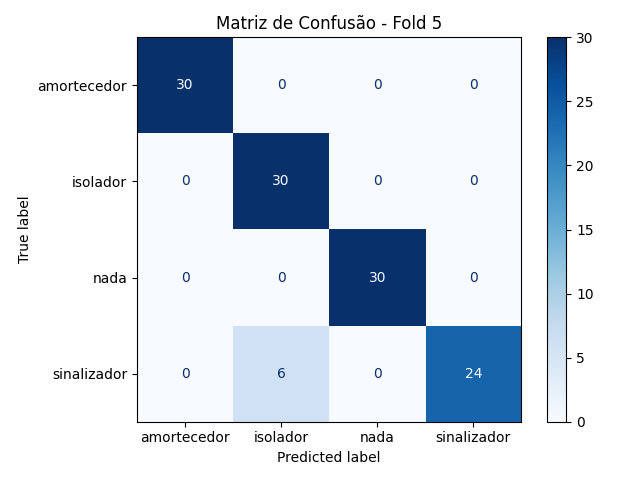
\includegraphics[width=0.7\linewidth]{figuras/Resultados/simu_principal_Teste2_knn.png}
\fonte{}
\label{fig:matriz_confusao_knn_lidar_bruto}
\end{figure}

\paragraph{Árvore de Decisão}

\begin{table}[H]
\centering
\caption{Desempenho da Árvore de Decisão com dados brutos do LiDAR (simulação)}
\label{tab:arvore_lidar_sim}
\begin{tabular}{ccccc}
\hline
\textbf{Dobra} & \textbf{Época Final} & \textbf{Perda Final} & \textbf{Acurácia (\%)} & \textbf{Tempo de Validação (s)} \\
\hline
1 & -  & -      & 100.00 & 0.0001 \\
2 & -  & -      & 99.17  & 0.0001 \\
3 & -  & -      & 99.17  & 0.0002 \\
4 & -  & -      & 100.00 & 0.0002 \\
5 & -  & -      & 99.17  & 0.0001 \\
\hline
\textbf{Média} & - & - & 99.50 & 0.0001 \\
\hline
\end{tabular} \fonte{}
\end{table}

\begin{figure}[H]
\caption{Árvore de decisão gerada para a dobra 1 utilizando dados brutos do LiDAR (simulação).}
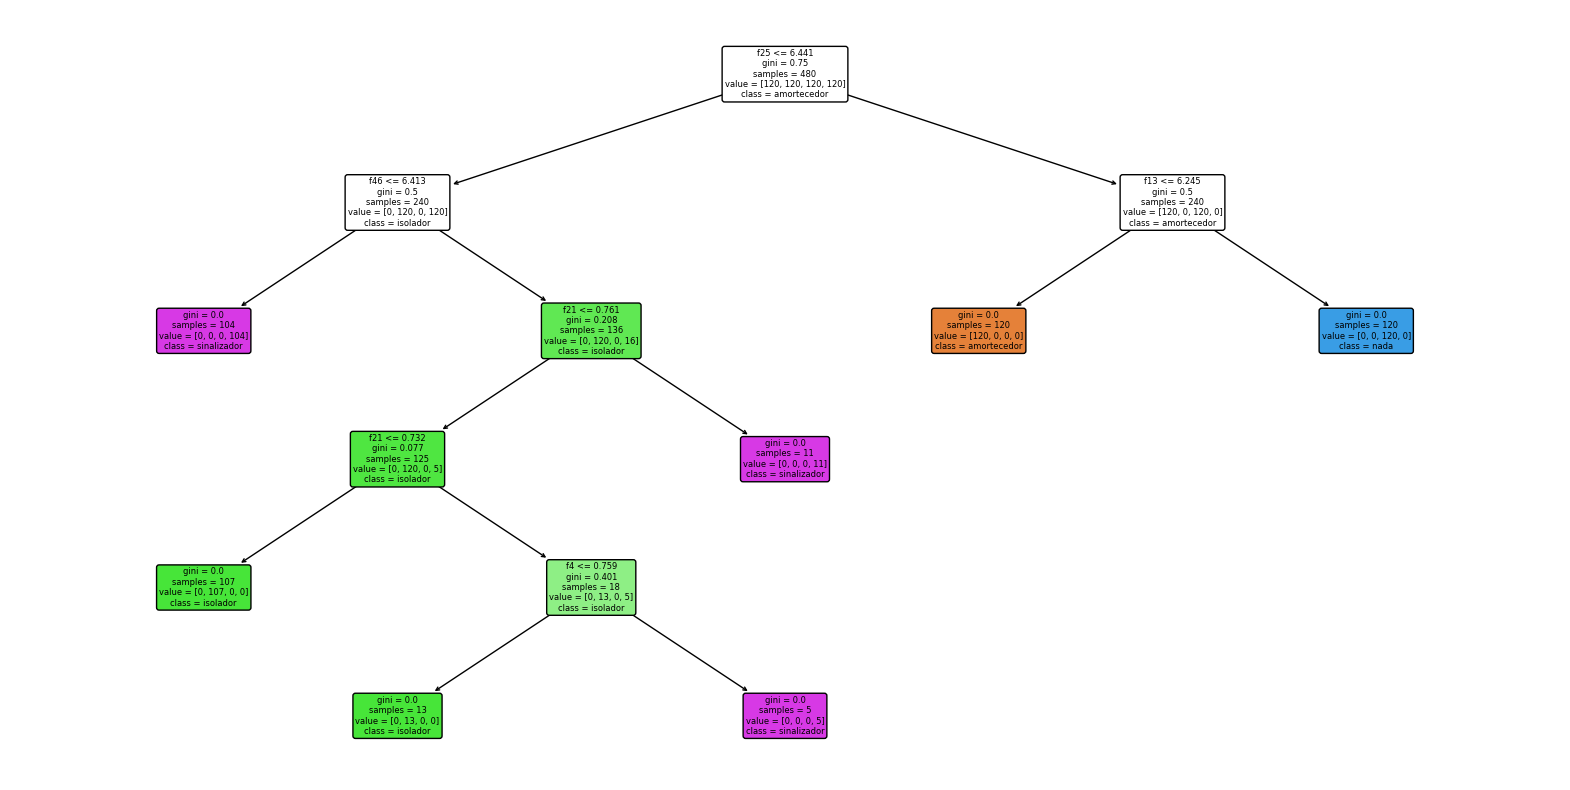
\includegraphics[width=0.9\textwidth]{figuras/Resultados/simu_principal_Teste2_arvore.png}
\fonte{}
\label{fig:arvore_decisao_dobra1}
\end{figure}


\paragraph{Naive Bayes}

\begin{table}[H]
\centering
\caption{Desempenho do Naive Bayes com dados brutos do LiDAR (simulação)}
\label{tab:naive_lidar_bruto}
\begin{tabular}{ccccc}
\hline
\textbf{Dobra} & \textbf{Época Final} & \textbf{Perda Final} & \textbf{Acurácia (\%)} & \textbf{Tempo de Validação (s)} \\
\hline
1 & - & --      & 99.17 & 0.0003 \\
2 & - & --      & 97.50 & 0.0005 \\
3 & - & --      & 97.50 & 0.0003 \\
4 & - & --      & 97.50 & 0.0003 \\
5 & - & --      & 93.33 & 0.0003 \\
\hline
\textbf{Média} & - & -- & 96.60 & 0.0003 \\
\hline
\end{tabular} \fonte{}
\end{table}

\begin{figure}[H]
\caption{Matriz de confusão do Naive Bayes na dobra 5 com dados brutos do LiDAR (simulação).}
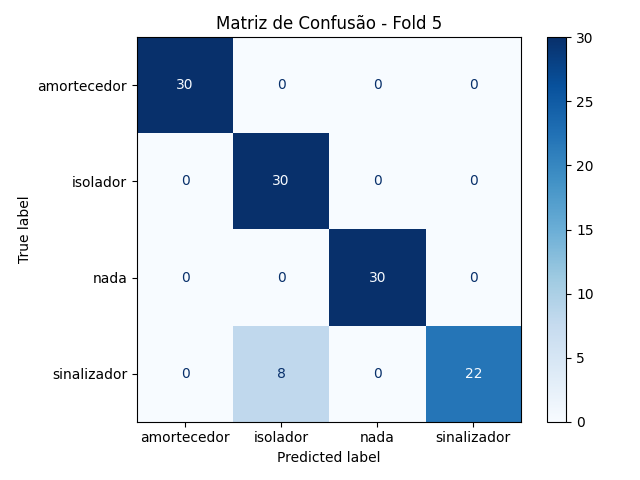
\includegraphics[width=0.7\linewidth]{figuras/Resultados/simu_principal_Teste2_naive.png}
\fonte{}
\label{fig:matriz_confusao_naive_lidar_bruto}
\end{figure}


\paragraph{Rede Neural}

\begin{table}[H]
\centering
\caption{Desempenho da Rede Neural com dados brutos do LiDAR (simulação)}
\label{tab:rede_neural_lidar_bruto}
\begin{tabular}{ccccc}
\hline
\textbf{Dobra} & \textbf{Época Final} & \textbf{Perda Final} & \textbf{Acurácia (\%)} & \textbf{Tempo de Validação (s)} \\
\hline
1 & 200 & 0.033461 & 96.67 & 0.0094 \\
2 & 200 & 0.025889 & 95.83 & 0.0021 \\
3 & 200 & 0.029690 & 98.33 & 0.0019 \\
4 & 200 & 0.029371 & 97.50 & 0.0019 \\
5 & 200 & 0.031941 & 93.33 & 0.0022 \\
\hline
\textbf{Média} & 200.0 & 0.030070 & 96.73 & 0.0035 \\
\hline
\end{tabular} \fonte{}
\end{table}

\begin{figure}[H]
\caption{Matriz de confusão da Rede Neural na dobra 2 com dados brutos do LiDAR (simulação).}
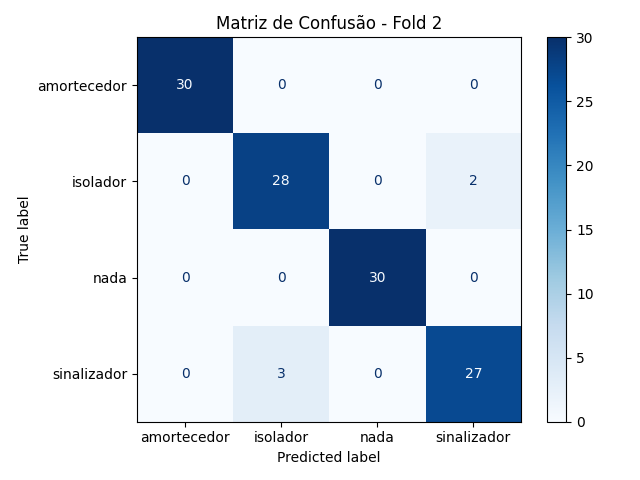
\includegraphics[width=0.7\linewidth]{figuras/Resultados/simu_principal_Teste2_nn.png}
\fonte{}
\label{fig:matriz_confusao_nn_lidar_bruto}
\end{figure}


\paragraph{Floresta Aleatória}

\begin{table}[!h]
\centering
\caption{Desempenho da Floresta Aleatória com dados brutos do LiDAR (simulação)}
\label{tab:rede_neural_features_imagem}
\begin{tabular}{ccccc}
\hline
\textbf{Dobra} & \textbf{Época Final} & \textbf{Perda Final} & \textbf{Acurácia (\%)} & \textbf{Tempo de Validação (s)} \\
\hline
1 & - & - & 100.0  & 0.0061 \\
2 & - & - & 99.17  & 0.0061 \\
3 & - & - & 99.17  & 0.0059 \\
4 & - & - & 100.0  & 0.0059 \\
5 & - & - & 100.0  & 0.0062 \\
\hline
\textbf{Média} & - & - & 99.7 & 0.0060 \\
\hline
\end{tabular} \fonte{}
\end{table}

\subsubsection{Features extraídas das imagens}

Esta subseção apresenta os resultados obtidos com o uso de \textit{features} extraídas das imagens de profundidade simuladas no robô principal. As imagens foram previamente processadas para extração de características numéricas representativas.

\paragraph{k-Vizinhos mais próximos}

\begin{table}[H]
\centering
\caption{Desempenho do k-Vizinhos mais próximos com features extraídas das imagens (simulação)}
\label{tab:knn_feat_img_simu}
\begin{tabular}{ccccc}
\hline
\textbf{Dobra} & \textbf{Época Final} & \textbf{Perda Final} & \textbf{Acurácia (\%)} & \textbf{Tempo de Validação (s)} \\
\hline
1 & - & - & 100.0 & 0.0029 \\
2 & - & - & 100.0 & 0.0054 \\
3 & - & - & 100.0 & 0.0027 \\
4 & - & - & 100.0 & 0.0028 \\
5 & - & - & 100.0 & 0.0028 \\
\hline
\textbf{Média} & - & - & 100.0 & 0.0033 \\
\hline
\end{tabular} \fonte{}
\end{table}

\paragraph{Árvore de Decisão}

\begin{table}[H]
\centering
\caption{Desempenho da Árvore de Decisão com features extraídas das imagens (simulação)}
\label{tab:tree_feat_img_simu}
\begin{tabular}{ccccc}
\hline
\textbf{Dobra} & \textbf{Época Final} & \textbf{Perda Final} & \textbf{Acurácia (\%)} & \textbf{Tempo de Validação (s)} \\
\hline
1 & - & - & 100.0 & 0.000138 \\
2 & - & - & 100.0 & 0.000123 \\
3 & - & - & 100.0 & 0.000124 \\
4 & - & - & 100.0 & 0.000124 \\
5 & - & - & 100.0 & 0.000124 \\
\hline
\textbf{Média} & - & - & 100.0 & 0.000127 \\
\hline
\end{tabular} \fonte{}
\end{table}

\paragraph{Naive Bayes}

\begin{table}[H]
\centering
\caption{Desempenho do Naive Bayes com features extraídas das imagens (simulação)}
\label{tab:naive_feat_img_simu}
\begin{tabular}{ccccc}
\hline
\textbf{Dobra} & \textbf{Época Final} & \textbf{Perda Final} & \textbf{Acurácia (\%)} & \textbf{Tempo de Validação (s)} \\
\hline
1 & - & - & 100.0 & 0.000209 \\
2 & - & - & 99.17 & 0.000212 \\
3 & - & - & 100.0 & 0.000194 \\
4 & - & - & 100.0 & 0.000211 \\
5 & - & - & 100.0 & 0.000214 \\
\hline
\textbf{Média} & - & - & 99.83 & 0.000208 \\
\hline
\end{tabular} \fonte{}
\end{table} 

\paragraph{Rede Neural}

\begin{table}[H]
\centering
\caption{Desempenho da Rede Neural com features extraídas das imagens (simulação)}
\label{tab:nn_feat_img_simu}
\begin{tabular}{ccccc}
\hline
\textbf{Dobra} & \textbf{Época Final} & \textbf{Perda Final} & \textbf{Acurácia (\%)} & \textbf{Tempo de Validação (s)} \\
\hline
1 & 79 & 0.000395 & 100.0 & 0.0117 \\
2 & 34 & 0.000362 & 100.0 & 0.0021 \\
3 & 63 & 0.000620 & 100.0 & 0.0024 \\
4 & 74 & 0.000415 & 99.17 & 0.0021 \\
5 & 49 & 0.000421 & 100.0 & 0.0025 \\
\hline
\textbf{Média} & 59.8 & 0.000443 & 99.83 & 0.0042 \\
\hline
\end{tabular} \fonte{}
\end{table}

\paragraph{Floresta Aleatória}

\begin{table}[H]
\centering
\caption{Desempenho da Floresta Aleatória com features extraídas das imagens (simulação)}
\label{tab:rf_feat_img_simu}
\begin{tabular}{ccccc}
\hline
\textbf{Dobra} & \textbf{Época Final} & \textbf{Perda Final} & \textbf{Acurácia (\%)} & \textbf{Tempo de Validação (s)} \\
\hline
1 & - & - & 100.0 & 0.0055 \\
2 & - & - & 100.0 & 0.0055 \\
3 & - & - & 100.0 & 0.0053 \\
4 & - & - & 100.0 & 0.0052 \\
5 & - & - & 100.0 & 0.0052 \\
\hline
\textbf{Média} & - & - & 100.0 & 0.0054 \\
\hline
\end{tabular} \fonte{}
\end{table}

\subsubsection{Features extraídas do LiDAR}

Esta subseção apresenta os resultados obtidos a partir de atributos derivados dos dados brutos de distância do sensor \textit{LiDAR}, coletados em simulações com o robô principal. As leituras foram processadas para extrair informações relevantes (\textit{features}) que pudessem melhorar a capacidade dos modelos de aprendizado de máquina.

\paragraph{k-Vizinhos mais próximos}

\begin{table}[H]
\centering
\caption{Desempenho do k-Vizinhos mais próximos com features extraídas do LiDAR (simulação)}
\label{tab:knn_features_lidar_simulado}
\begin{tabular}{ccccc}
\hline
\textbf{Dobra} & \textbf{Época Final} & \textbf{Perda Final} & \textbf{Acurácia (\%)} & \textbf{Tempo de Validação (s)} \\
\hline
1 & - & - & 97.5  & 0.0027 \\
2 & - & - & 95.0  & 0.0026 \\
3 & - & - & 96.67 & 0.0030 \\
4 & - & - & 96.67 & 0.0029 \\
5 & - & - & 93.33 & 0.0028 \\
\hline
\textbf{Média} & - & - & 95.83 & 0.0028 \\
\hline
\end{tabular} \fonte{}
\end{table}

\begin{figure}[H]
\caption{Matriz de confusão do k-Vizinhos mais próximos na dobra 5 com features extraídas do LiDAR (simulação).}
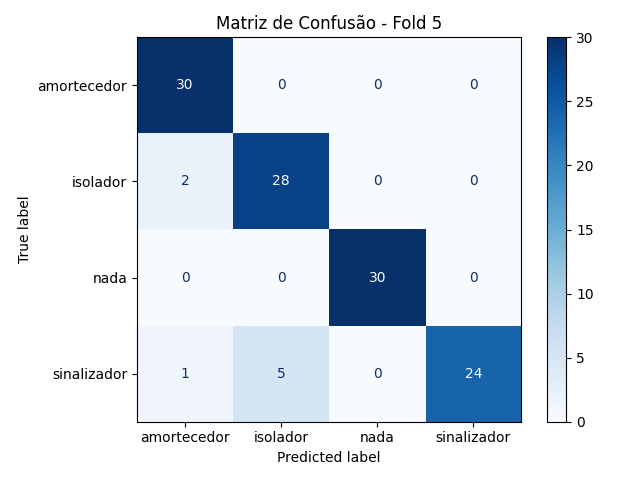
\includegraphics[width=0.7\linewidth]{figuras/Resultados/simu_principal_Teste4_knn.png}
\fonte{}
\label{fig:matriz_confusao_knn_lidar_features}
\end{figure}


\paragraph{Árvore de Decisão}

\begin{table}[H]
\centering
\caption{Desempenho da Árvore de Decisão com features extraídas do LiDAR (simulação)}
\label{tab:arvore_features_lidar_simulado}
\begin{tabular}{ccccc}
\hline
\textbf{Dobra} & \textbf{Época Final} & \textbf{Perda Final} & \textbf{Acurácia (\%)} & \textbf{Tempo de Validação (s)} \\
\hline
1 & - & - & 98.33 & 0.0001 \\
2 & - & - & 98.33 & 0.0002 \\
3 & - & - & 99.17 & 0.0001 \\
4 & - & - & 98.33 & 0.0001 \\
5 & - & - & 96.67 & 0.0002 \\
\hline
\textbf{Média} & - & - & 98.17 & 0.0001 \\
\hline
\end{tabular} \fonte{}
\end{table}

\paragraph{Naive Bayes}

\begin{table}[H]
\centering
\caption{Desempenho do Naive Bayes com features extraídas do LiDAR (simulação)}
\label{tab:naive_features_lidar_simulado}
\begin{tabular}{ccccc}
\hline
\textbf{Dobra} & \textbf{Época Final} & \textbf{Perda Final} & \textbf{Acurácia (\%)} & \textbf{Tempo de Validação (s)} \\
\hline
1 & - & - & 94.17 & 0.00022 \\
2 & - & - & 95.00 & 0.00021 \\
3 & - & - & 94.17 & 0.00034 \\
4 & - & - & 95.00 & 0.00033 \\
5 & - & - & 90.00 & 0.00020 \\
\hline
\textbf{Média} & - & - & 93.67 & 0.00026 \\
\hline
\end{tabular} \fonte{}
\end{table}

\begin{figure}[H]
\caption{Matriz de confusão do Naive Bayes na dobra 5 com features extraídas do LiDAR (simulação).}
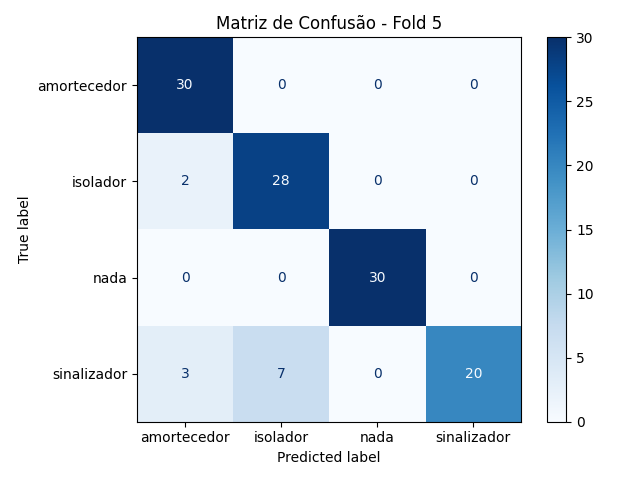
\includegraphics[width=0.7\linewidth]{figuras/Resultados/simu_principal_Teste4_naive.png}
\fonte{}
\label{fig:matriz_confusao_naive_lidar_features}
\end{figure}

\paragraph{Rede Neural}

\begin{table}[H]
\centering
\caption{Desempenho da Rede Neural com features extraídas do LiDAR (simulação)}
\label{tab:rede_neural_lidar_features}
\begin{tabular}{ccccc}
\hline
\textbf{Dobra} & \textbf{Época Final} & \textbf{Perda Final} & \textbf{Acurácia (\%)} & \textbf{Tempo de Validação (s)} \\
\hline
1 & 200 & 0.214619 & 95.00 & 0.00914 \\
2 & 200 & 0.203636 & 94.17 & 0.00183 \\
3 & 200 & 0.202239 & 93.33 & 0.00210 \\
4 & 200 & 0.223546 & 95.83 & 0.00187 \\
5 & 200 & 0.213401 & 89.17 & 0.00193 \\
\hline
\textbf{Média} & 200 & 0.211088 & 93.90 & 0.00377 \\
\hline
\end{tabular}
\fonte{}
\end{table}

\begin{figure}[H]
\caption{Matriz de confusão da Rede Neural na dobra 5 com features extraídas do LiDAR (simulação).}
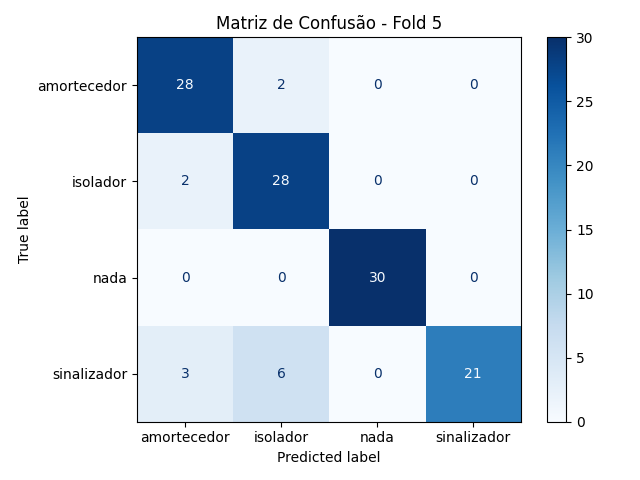
\includegraphics[width=0.7\linewidth]{figuras/Resultados/simu_principal_Teste4_nn.png}
\fonte{}
\label{fig:matriz_confusao_nn_lidar_features}
\end{figure}


\paragraph{Floresta Aleatória}

\begin{table}[H]
\centering
\caption{Desempenho da Floresta Aleatória com features extraídas do LiDAR (simulação)}
\label{tab:floresta_aleatoria_lidar_features}
\begin{tabular}{ccccc}
\hline
\textbf{Dobra} & \textbf{Época Final} & \textbf{Perda Final} & \textbf{Acurácia (\%)} & \textbf{Tempo de Validação (s)} \\
\hline
1 & -   & -        & 98.33 & 0.00586 \\
2 & -   & -        & 95.00 & 0.00551 \\
3 & -   & -        & 98.33 & 0.00582 \\
4 & -   & -        & 98.33 & 0.00550 \\
5 & -   & -        & 97.50 & 0.00572 \\
\hline
\textbf{Média} & - & - & 97.50 & 0.00566 \\
\hline
\end{tabular}
\fonte{}
\end{table}

\subsubsection{Features combinadas}

Esta subseção apresenta os resultados obtidos a partir da combinação das \textit{features} extraídas das imagens e dos dados do sensor \textit{LiDAR}, coletados em simulações com o robô principal.

\paragraph{k-Vizinhos mais próximos}

\begin{table}[H]
\centering
\caption{Desempenho do k-Vizinhos mais próximos com features combinadas (simulação)}
\label{tab:knn_features_combinadas}
\begin{tabular}{ccccc}
\hline
\textbf{Dobra} & \textbf{Época Final} & \textbf{Perda Final} & \textbf{Acurácia (\%)} & \textbf{Tempo de Validação (s)} \\
\hline
1 & - & -       & 100.0 & 0.0027 \\
2 & - & -       & 100.0 & 0.0028 \\
3 & - & -       & 100.0 & 0.0029 \\
4 & - & -       & 100.0 & 0.0027 \\
5 & - & -       & 100.0 & 0.0030 \\
\hline
\textbf{Média} & 1 & -      & 100.0 & 0.00282 \\
\hline
\end{tabular}
\fonte{}
\end{table}

\paragraph{Árvore de Decisão}

\begin{table}[H]
\centering
\caption{Desempenho da Árvore de Decisão com features combinadas (simulação)}
\label{tab:arvore_features_combinadas}
\begin{tabular}{ccccc}
\hline
\textbf{Dobra} & \textbf{Época Final} & \textbf{Perda Final} & \textbf{Acurácia (\%)} & \textbf{Tempo de Validação (s)} \\
\hline
1 & - & -       & 100.0 & 0.000137 \\
2 & - & -       & 100.0 & 0.000128 \\
3 & - & -       & 100.0 & 0.000121 \\
4 & - & -       & 100.0 & 0.000174 \\
5 & - & -       & 100.0 & 0.000122 \\
\hline
\textbf{Média} & 1 & -      & 100.0 & 0.000136 \\
\hline
\end{tabular}
\fonte{}
\end{table}

\paragraph{Naive Bayes}

\begin{table}[H]
\centering
\caption{Desempenho do Naive Bayes com features combinadas (simulação)}
\label{tab:naive_bayes_features_combinadas}
\begin{tabular}{ccccc}
\hline
\textbf{Dobra} & \textbf{Época Final} & \textbf{Perda Final} & \textbf{Acurácia (\%)} & \textbf{Tempo de Validação (s)} \\
\hline
1 & - & -       & 100.0 & 0.000205 \\
2 & - & -       & 99.17 & 0.000200 \\
3 & - & -       & 100.0 & 0.000215 \\
4 & - & -       & 100.0 & 0.000197 \\
5 & - & -       & 100.0 & 0.000232 \\
\hline
\textbf{Média} & 1 & -      & 99.83 & 0.000210 \\
\hline
\end{tabular}
\fonte{}
\end{table}


\paragraph{Rede Neural}

\begin{table}[H]
\centering
\caption{Desempenho da Rede Neural com features combinadas (simulação)}
\label{tab:rn_features_lidar}
\begin{tabular}{ccccc}
\hline
\textbf{Dobra} & \textbf{Época Final} & \textbf{Perda Final} & \textbf{Acurácia (\%)} & \textbf{Tempo de Validação (s)} \\
\hline
1 & 49  & 0.000374 & 100.0  & 0.0096 \\
2 & 66  & 0.000453 & 99.17  & 0.0022 \\
3 & 98  & 0.000035 & 100.0  & 0.0023 \\
4 & 75  & 0.000934 & 100.0  & 0.0019 \\
5 & 38  & 0.000445 & 100.0  & 0.0020 \\
\hline
\textbf{Média} & 65.2 & 0.000428 & 99.67 & 0.0036 \\
\hline
\end{tabular}
\fonte{}
\end{table}

\paragraph{Floresta Aleatória}

\begin{table}[H]
\centering
\caption{Desempenho da Floresta Aleatória com features combinadas (simulação)}
\label{tab:floresta_features_lidar}
\begin{tabular}{ccccc}
\hline
\textbf{Dobra} & \textbf{Época Final} & \textbf{Perda Final} & \textbf{Acurácia (\%)} & \textbf{Tempo de Validação (s)} \\
\hline
1 & - & - & 100.0 & 0.0057 \\
2 & - & - & 100.0 & 0.0053 \\
3 & - & - & 100.0 & 0.0057 \\
4 & - & - & 100.0 & 0.0058 \\
5 & - & - & 100.0 & 0.0054 \\
\hline
\textbf{Média} & - & - & 100.0 & 0.0056 \\
\hline
\end{tabular}
\fonte{}
\end{table}

\subsection{Dados reais}

Nesta subseção são apresentados os resultados obtidos a partir dos dados reais gerados pelo robô principal durante as execuções no ambiente do laboratório.

\subsubsection{Imagens brutas}

Esta subseção apresenta os resultados obtidos com as imagens de profundidade brutas capturadas pelo robô principal em ambiente real no laboratório.

\begin{table}[H]
\centering
\caption{Desempenho da SqueezeNet com imagens brutas (real)}
\label{tab:squeezenet_lidar_real}
\begin{tabular}{ccccc}
\hline
\textbf{Dobra} & \textbf{Época Final} & \textbf{Perda Final} & \textbf{Acurácia (\%)} & \textbf{Tempo de Validação (s)} \\
\hline
1 & 10 & 0.000032 & 100.0 & 0.7084 \\
2 & 11 & 0.000280 & 100.0 & 0.6005 \\
3 & 9  & 0.000295 & 100.0 & 0.6091 \\
4 & 2  & 0.000004 & 100.0 & 0.6110 \\
5 & 4  & 0.000735 & 100.0 & 0.6307 \\
\hline
\textbf{Média} & 7.2 & 0.000269 & 100.0 & 0.6319 \\
\hline
\end{tabular}
\fonte{}
\end{table}

\subsubsection{Dados brutos do LiDAR}

Esta subseção apresenta os resultados obtidos diretamente dos dados brutos de distância fornecidos pelo sensor \textit{LiDAR}, coletados em ambientes reais com o robô principal. 

\paragraph{k-Vizinhos mais próximos}

\begin{table}[H]
\centering
\caption{Desempenho do k-Vizinhos mais próximos com dados brutos do LiDAR (real)}
\label{tab:knn_lidar_bruto_real_2}
\begin{tabular}{ccccc}
\hline
\textbf{Dobra} & \textbf{Época Final} & \textbf{Perda Final} & \textbf{Acurácia (\%)} & \textbf{Tempo de Validação (s)} \\
\hline
1 & - & - & 87.50 & 0.0039 \\
2 & - & - & 93.33 & 0.0037 \\
3 & - & - & 93.33 & 0.0031 \\
4 & - & - & 91.67 & 0.0032 \\
5 & - & - & 86.67 & 0.0034 \\
\hline
\textbf{Média} & - & - & 90.90 & 0.00346 \\
\hline
\end{tabular}
\fonte{}
\end{table}

\begin{figure}[H]
\caption{Matriz de confusão do k-Vizinhos mais próximos na dobra 1 com dados brutos do LiDAR (real).}
\centering
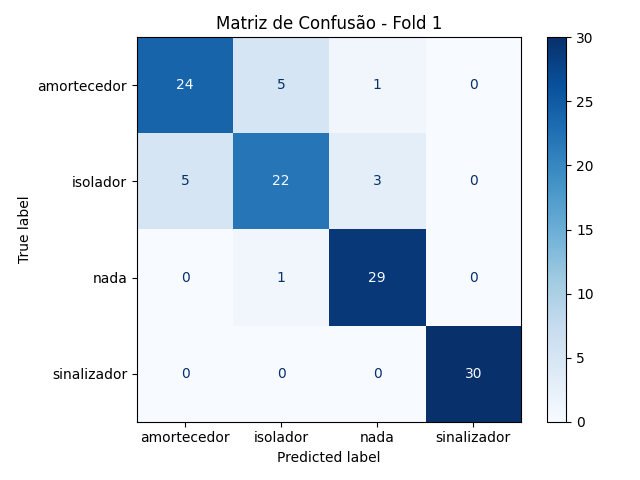
\includegraphics[width=0.7\linewidth]{figuras/Resultados/real_principal_Teste2_knn.png}
\fonte{}
\label{fig:matriz_confusao_knn_lidar_bruto_real}
\end{figure}


\paragraph{Árvore de Decisão}

\begin{table}[H]
\centering
\caption{Desempenho do Árvore de Decisão com dados brutos do LiDAR (real)}
\label{tab:arvore_lidar_bruto_real_2}
\begin{tabular}{ccccc}
\hline
\textbf{Dobra} & \textbf{Época Final} & \textbf{Perda Final} & \textbf{Acurácia (\%)} & \textbf{Tempo de Validação (s)} \\
\hline
1 & - & - & 100.00 & 0.000144 \\
2 & - & - & 99.17 & 0.000139 \\
3 & - & - & 100.00 & 0.000136 \\
4 & - & - & 99.17 & 0.000215 \\
5 & - & - & 97.50 & 0.000159 \\
\hline
\textbf{Média} & - & - & 99.37 & 0.000159 \\
\hline
\end{tabular}
\fonte{}
\end{table}

\paragraph{Naive Bayes}

\begin{table}[H]
\centering
\caption{Desempenho do Naive Bayes com dados brutos do LiDAR (real)}
\label{tab:naive_lidar_bruto_real}
\begin{tabular}{ccccc}
\hline
\textbf{Dobra} & \textbf{Época Final} & \textbf{Perda Final} & \textbf{Acurácia (\%)} & \textbf{Tempo de Validação (s)} \\
\hline
1 & - & - & 86.67 & 0.000273 \\
2 & - & - & 80.83 & 0.000262 \\
3 & - & - & 81.67 & 0.000290 \\
4 & - & - & 80.00 & 0.000286 \\
5 & - & - & 77.50 & 0.000270 \\
\hline
\textbf{Média} & - & - & 81.33 & 0.000276 \\
\hline
\end{tabular}
\fonte{}
\end{table}

\begin{figure}[H]
\caption{Matriz de confusão do Naive Bayes na dobra 2 com dados brutos do LiDAR (real).}
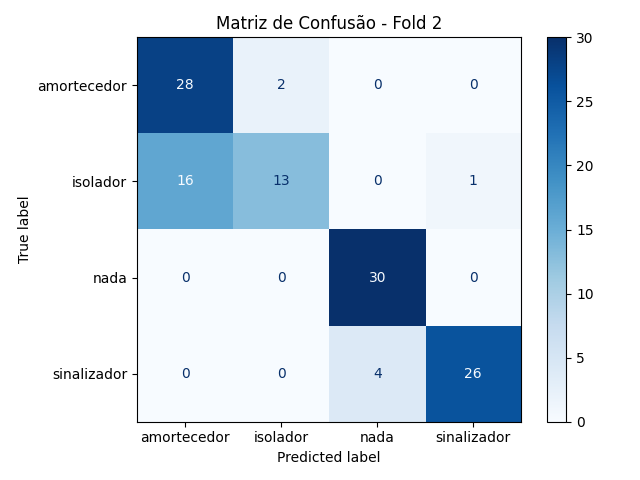
\includegraphics[width=0.7\linewidth]{figuras/Resultados/real_principal_Teste2_naive.png}
\fonte{}
\label{fig:matriz_confusao_naive_lidar_real_dobra2}
\end{figure}

\paragraph{Rede Neural}

\begin{table}[H]
\centering
\caption{Desempenho da Rede Neural com dados brutos do LiDAR (real)}
\label{tab:nn_lidar_bruto_real}
\begin{tabular}{ccccc}
\hline
\textbf{Dobra} & \textbf{Época Final} & \textbf{Perda Final} & \textbf{Acurácia (\%)} & \textbf{Tempo de Validação (s)} \\
\hline
1 & 200 & 0.003282 & 93.33 & 0.010296 \\
2 & 200 & 0.004890 & 94.17 & 0.003278 \\
3 & 200 & 0.004671 & 93.33 & 0.001895 \\
4 & 160 & 0.000999 & 94.17 & 0.001972 \\
5 & 200 & 0.004385 & 90.83 & 0.001836 \\
\hline
\textbf{Média} & 192 & 0.003645 & 93.17 & 0.003855 \\
\hline
\end{tabular}
\fonte{}
\end{table}

\begin{figure}[H]
\caption{Matriz de confusão da Rede Neural na dobra 5 com dados brutos do LiDAR (real).}
\centering
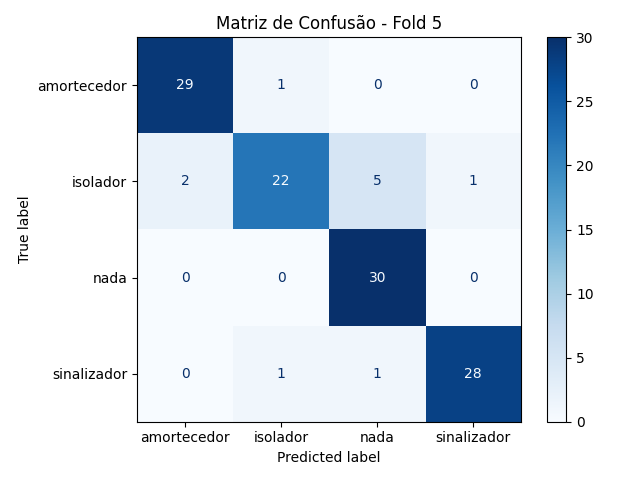
\includegraphics[width=0.7\linewidth]{figuras/Resultados/real_principal_Teste2_nn.png}
\fonte{}
\label{fig:matriz_confusao_nn_lidar_bruto_real}
\end{figure}

\paragraph{Floresta Aleatória}

\begin{table}[H]
\centering
\caption{Desempenho da Floresta Aleatória com dados brutos do LiDAR (real)}
\label{tab:rf_lidar_bruto_real}
\begin{tabular}{ccccc}
\hline
\textbf{Dobra} & \textbf{Época Final} & \textbf{Perda Final} & \textbf{Acurácia (\%)} & \textbf{Tempo de Validação (s)} \\
\hline
1 & - & - & 100.0 & 0.005681 \\
2 & - & - & 100.0 & 0.005755 \\
3 & - & - & 100.0 & 0.005916 \\
4 & - & - & 100.0 & 0.006184 \\
5 & - & - & 100.0 & 0.006251 \\
\hline
\textbf{Média} & - & - & 100.0 & 0.005957 \\
\hline
\end{tabular}
\fonte{}
\end{table}

\subsubsection{Features extraídas das imagens}

Esta subseção apresenta os resultados obtidos a partir de atributos derivados das imagens reais coletadas pelo robô principal. As imagens foram processadas para extrair informações relevantes (\textit{features}) que pudessem melhorar a capacidade dos modelos de aprendizado de máquina na identificação das classes de objetos.

\paragraph{k-Vizinhos mais próximos}

\begin{table}[H]
\caption{Desempenho do k-Vizinhos mais próximos com features extraídas das imagens (real).}
\centering
\begin{tabular}{ccccc}
\hline
\textbf{Dobra} & \textbf{Época Final} & \textbf{Perda Final} & \textbf{Acurácia (\%)} & \textbf{Tempo de Validação (s)}  \\
\hline
1 & - & - & 100,0 & 0,0030 \\
2 & - & - & 100,0 & 0,0030 \\
3 & - & - & 100,0 & 0,0029 \\
4 & - & - & 100,0 & 0,0030 \\
5 & - & - & 100,0 & 0,0031 \\
\hline
\textbf{Média} & - & - & 100,0 & 0,0030 \\
\hline
\end{tabular}
\fonte{}
\label{tab:knn_features_imagens}
\end{table} 

\paragraph{Árvore de Decisão}

\begin{table}[H]
\caption{Desempenho da Árvore de Decisão com features extraídas das imagens (real).}
\centering
\begin{tabular}{ccccc}
\hline
\textbf{Dobra} & \textbf{Época Final} & \textbf{Perda Final} & \textbf{Acurácia (\%)} & \textbf{Tempo de Validação (s)}  \\
\hline
1 & - & - & 100,0 & 0,000154 \\
2 & - & - & 100,0 & 0,000129 \\
3 & - & - & 100,0 & 0,000138 \\
4 & - & - & 100,0 & 0,000135 \\
5 & - & - & 99,17 & 0,000128 \\
\hline
\textbf{Média} & - & - & 99,67 & 0,000137 \\
\hline
\end{tabular}
\fonte{}
\label{tab:arvore_features_imagens}
\end{table}

\paragraph{Naive Bayes}

\begin{table}[H]
\caption{Desempenho do Naive Bayes com features extraídas das imagens (real).}
\centering
\begin{tabular}{ccccc}
\hline
\textbf{Dobra} & \textbf{Época Final} & \textbf{Perda Final} & \textbf{Acurácia (\%)} & \textbf{Tempo de Validação (s)}  \\
\hline
1 & - & - & 99,17 & 0,000196 \\
2 & - & - & 100,0 & 0,000192 \\
3 & - & - & 99,17 & 0,000350 \\
4 & - & - & 100,0 & 0,000243 \\
5 & - & - & 98,33 & 0,000200 \\
\hline
\textbf{Média} & - & - & 99,33 & 0,000236 \\
\hline
\end{tabular}
\fonte{}
\label{tab:naive_features_imagens}
\end{table}


\paragraph{Rede Neural}

\begin{table}[H]
\caption{Desempenho da Rede Neural com features extraídas das imagens (real).}
\centering
\begin{tabular}{ccccc}
\hline
\textbf{Dobra} & \textbf{Época Final} & \textbf{Perda Final} & \textbf{Acurácia (\%)} & \textbf{Tempo de Validação (s)}  \\
\hline
1 & 200 & 7,458555 & 89,17 & 0,009501 \\
2 & 200 & 1,502896 & 87,5 & 0,001873 \\
3 & 200 & 3,814955 & 89,17 & 0,001903 \\
4 & 200 & 10,270095 & 86,67 & 0,001998 \\
5 & 200 & 4,025579 & 86,67 & 0,001852 \\
\hline
\textbf{Média} & 200 & 5,014204 & 87,84 & 0,003025 \\
\hline
\end{tabular}
\fonte{}
\label{tab:rn_features_imagens_real}
\end{table}

\begin{figure}[H]
\caption{Matriz de confusão da Rede Neural na dobra 4 com features extraídas das imagens (real).}
\centering
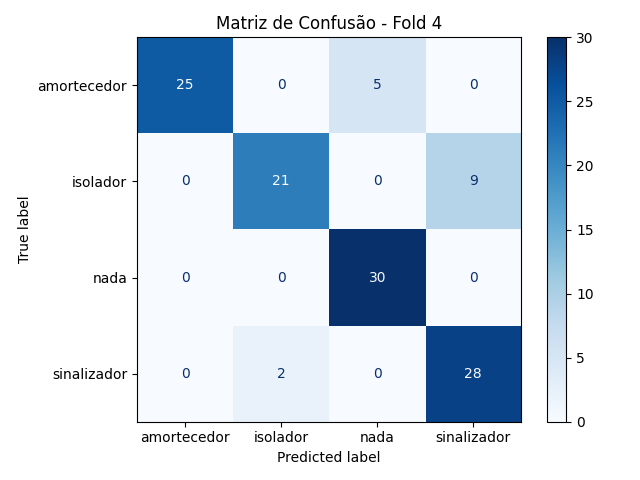
\includegraphics[width=0.7\linewidth]{figuras/Resultados/real_principal_Teste3_nn.png}
\fonte{}
\label{fig:matriz_confusao_rn_imagens_real}
\end{figure}


\paragraph{Floresta Aleatória}

\begin{table}[H]
\caption{Desempenho da Floresta Aleatória com features extraídas das imagens (real).}
\centering
\begin{tabular}{ccccc}
\hline
\textbf{Dobra} & \textbf{Época Final} & \textbf{Perda Final} & \textbf{Acurácia (\%)} & \textbf{Tempo de Validação (s)}  \\
\hline
1 & - & - & 99,17 & 0,005706 \\
2 & - & - & 100,0 & 0,005852 \\
3 & - & - & 100,0 & 0,005603 \\
4 & - & - & 100,0 & 0,005454 \\
5 & - & - & 100,0 & 0,005498 \\
\hline
\textbf{Média} & - & - & 99,67 & 0,005623 \\
\hline
\end{tabular}
\fonte{}
\label{tab:rf_features_imagens_real}
\end{table}


\subsubsection{Features extraídas do LiDAR}

Esta subseção apresenta os resultados obtidos a partir de atributos derivados dos dados brutos reais de distância do sensor \textit{LiDAR}, coletados com o robô principal. As leituras foram processadas para extrair informações relevantes (\textit{features}) que pudessem melhorar a capacidade dos modelos de aprendizado de máquina.

\paragraph{k-Vizinhos mais próximos}

\begin{table}[H]
\caption{Desempenho do k-Vizinhos mais próximos com features extraídas do LiDAR (real).}
\centering
\begin{tabular}{ccccc}
\hline
\textbf{Dobra} & \textbf{Época Final} & \textbf{Perda Final} & \textbf{Acurácia (\%)} & \textbf{Tempo de Validação (s)}  \\
\hline
1 & - & - & 91,67 & 0,0030 \\
2 & - & - & 94,17 & 0,0027 \\
3 & - & - & 94,17 & 0,0028 \\
4 & - & - & 95,83 & 0,0028 \\
5 & - & - & 90,00 & 0,0027 \\
\hline
\textbf{Média} & - & - & 93,17 & 0,0028 \\
\hline
\end{tabular}
\fonte{}
\label{tab:knn_features_imagens_real}
\end{table}

\begin{figure}[H]
\caption{Matriz de confusão do k-Vizinhos mais próximos na dobra 5 com features extraídas do LiDAR (real).}
\centering
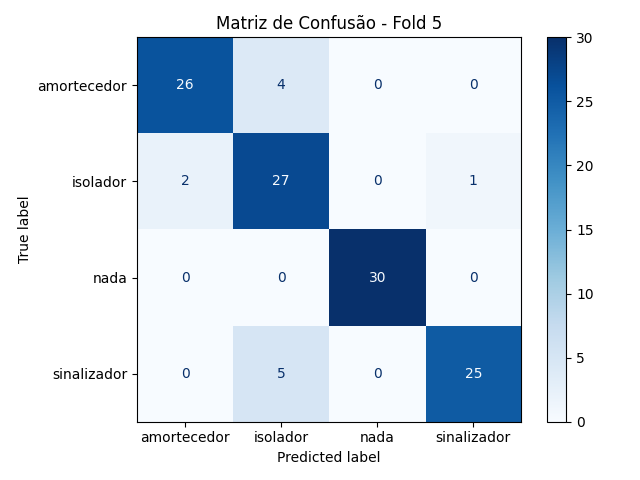
\includegraphics[width=0.7\linewidth]{figuras/Resultados/real_principal_Teste4_knn.png}
\fonte{}
\label{fig:matriz_confusao_knn_imagens_real_dobra5}
\end{figure}

\paragraph{Árvore de Decisão}

\begin{table}[H]
\caption{Desempenho da Árvore de Decisão com features extraídas do LiDAR (real).}
\centering
\begin{tabular}{ccccc}
\hline
\textbf{Dobra} & \textbf{Época Final} & \textbf{Perda Final} & \textbf{Acurácia (\%)} & \textbf{Tempo de Validação (s)}  \\
\hline
1 & - & - & 97,50 & 0,000133 \\
2 & - & - & 99,17 & 0,000135 \\
3 & - & - & 97,50 & 0,000124 \\
4 & - & - & 98,33 & 0,000137 \\
5 & - & - & 95,00 & 0,000138 \\
\hline
\textbf{Média} & - & - & 97,50 & 0,000134 \\
\hline
\end{tabular}
\fonte{}
\label{tab:arvore_decisao_features_imagens_real}
\end{table}

\paragraph{Naive Bayes}

\begin{table}[H]
\caption{Desempenho do Naive Bayes com features extraídas do LiDAR (real).}
\centering
\begin{tabular}{ccccc}
\hline
\textbf{Dobra} & \textbf{Época Final} & \textbf{Perda Final} & \textbf{Acurácia (\%)} & \textbf{Tempo de Validação (s)}  \\
\hline
1 & - & - & 96,67 & 0,00026 \\
2 & - & - & 94,17 & 0,000252 \\
3 & - & - & 93,33 & 0,000207 \\
4 & - & - & 93,33 & 0,000205 \\
5 & - & - & 90,00 & 0,000295 \\
\hline
\textbf{Média} & - & - & 93,90 & 0,000244 \\
\hline
\end{tabular}
\fonte{}
\label{tab:naive_bayes_features_imagens_real}
\end{table}

\begin{figure}[H]
\caption{Matriz de confusão do Naive Bayes na dobra 5 com features extraídas do LiDAR (real).}
\centering
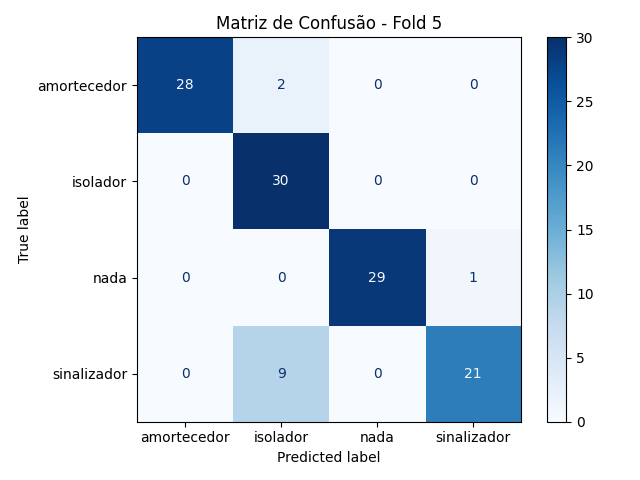
\includegraphics[width=0.7\linewidth]{figuras/Resultados/real_principal_Teste4_naive.png}
\fonte{}
\label{fig:matriz_confusao_naive_imagens_real}
\end{figure}

\paragraph{Rede Neural}

\begin{table}[H]
\caption{Desempenho da Rede Neural com features extraídas do LiDAR (real).}
\centering
\begin{tabular}{ccccc}
\hline
\textbf{Dobra} & \textbf{Época Final} & \textbf{Perda Final} & \textbf{Acurácia (\%)} & \textbf{Tempo de Validação (s)}  \\
\hline
1 & 200 & 0.135437 & 96.67 & 0.010137 \\
2 & 200 & 0.121473 & 95.83 & 0.002069 \\
3 & 200 & 0.143646 & 95.83 & 0.002144 \\
4 & 200 & 0.109989 & 96.67 & 0.002189 \\
5 & 200 & 0.168874 & 90.00 & 0.001935 \\
\hline
\multicolumn{3}{c}{Média} & 95.00 & 0.003295 \\
\hline
\end{tabular}
\fonte{}
\label{tab:resultados_nn_imagens_real}
\end{table}

\begin{figure}[H]
\caption{Matriz de confusão da Rede Neural na dobra 5 com features extraídas do LiDAR (real).}
\centering
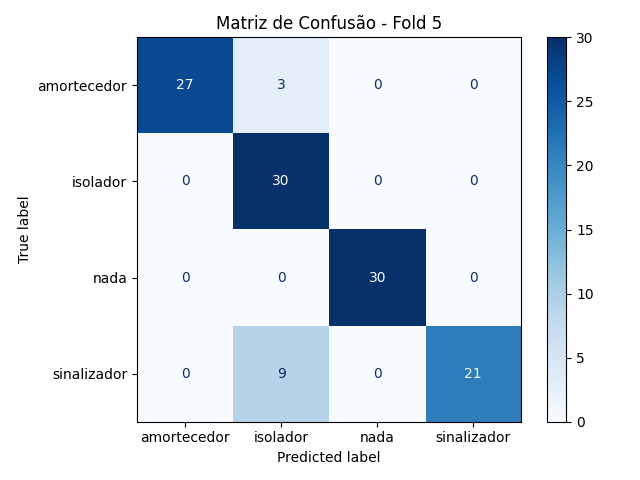
\includegraphics[width=0.7\linewidth]{figuras/Resultados/real_principal_Teste4_nn.png}
\fonte{}
\label{fig:matriz_confusao_nn_imagens_real}
\end{figure}


\paragraph{Floresta Aleatória}

\begin{table}[H]
\caption{Desempenho da Floresta Aleatória com features extraídas do LiDAR (real).}
\centering
\begin{tabular}{ccccc}
\hline
\textbf{Dobra} & \textbf{Época Final} & \textbf{Perda Final} & \textbf{Acurácia (\%)} & \textbf{Tempo de Validação (s)}  \\
\hline
1 & - & - & 100.0 & 0.005577 \\
2 & - & - & 98.33 & 0.005834 \\
3 & - & - & 99.17 & 0.006009 \\
4 & - & - & 96.67 & 0.005491 \\
5 & - & - & 97.5 & 0.005741 \\
\hline
\multicolumn{3}{c}{Média} & 98.33 & 0.005730 \\
\hline
\end{tabular}
\fonte{}
\label{tab:resultados_rf_imagens_real}
\end{table}


\subsubsection{Features combinadas}

Esta subseção apresenta os resultados obtidos a partir da combinação das \textit{features} extraídas das imagens e dos dados do sensor \textit{LiDAR} reais, coletados com o robô principal.

\paragraph{k-Vizinhos mais próximos}

\begin{table}[H]
\caption{Desempenho do k-Vizinhos mais próximos com features combinadas (real).}
\centering
\begin{tabular}{ccccc}
\hline
\textbf{Dobra} & \textbf{Época Final} & \textbf{Perda Final} & \textbf{Acurácia (\%)} & \textbf{Tempo de Validação (s)}  \\
\hline
1 & - & - & 100.0 & 0.0028 \\
2 & - & - & 100.0 & 0.0028 \\
3 & - & - & 100.0 & 0.0029 \\
4 & - & - & 100.0 & 0.0028 \\
5 & - & - & 100.0 & 0.0031 \\
\hline
\multicolumn{3}{c}{Média} & 100.0 & 0.0029 \\
\hline
\end{tabular}
\fonte{}
\label{tab:resultados_knn_imagens_real}
\end{table}


\paragraph{Árvore de Decisão}

\begin{table}[H]
\caption{Desempenho do Naive Bayes com features combinadas (real).}
\centering
\begin{tabular}{ccccc}
\hline
\textbf{Dobra} & \textbf{Época Final} & \textbf{Perda Final} & \textbf{Acurácia (\%)} & \textbf{Tempo de Validação (s)}  \\
\hline
1 & - & - & 100.0 & 0.000131 \\
2 & - & - & 100.0 & 0.000139 \\
3 & - & - & 100.0 & 0.000138 \\
4 & - & - & 98.33 & 0.000134 \\
5 & - & - & 99.17 & 0.000134 \\
\hline
\multicolumn{3}{c}{Média} & 99.5 & 0.000134 \\
\hline
\end{tabular}
\fonte{}
\label{tab:resultados_naive_imagens_real}
\end{table}

\paragraph{Naive Bayes}

\begin{table}[H]
\caption{Desempenho do Naive Bayes com features combinadas (real).}
\centering
\begin{tabular}{ccccc}
\hline
\textbf{Dobra} & \textbf{Época Final} & \textbf{Perda Final} & \textbf{Acurácia (\%)} & \textbf{Tempo de Validação (s)}  \\
\hline
1 & - & - & 100.0 & 0.000224 \\
2 & - & - & 100.0 & 0.000198 \\
3 & - & - & 100.0 & 0.000210 \\
4 & - & - & 100.0 & 0.000235 \\
5 & - & - & 98.33 & 0.000205 \\
\hline
\multicolumn{3}{c}{Média} & 99.67 & 0.000214 \\
\hline
\end{tabular}
\fonte{}
\label{tab:resultados_naive_lidar_real}
\end{table}

\paragraph{Rede Neural}

\begin{table}[H]
\caption{Desempenho da Rede Neural com features combinadas (real).}
\centering
\begin{tabular}{ccccc}
\hline
\textbf{Dobra} & \textbf{Época Final} & \textbf{Perda Final} & \textbf{Acurácia (\%)} & \textbf{Tempo de Validação (s)}  \\
\hline
1 & 200 & 1.0448 & 94.17 & 0.009344 \\
2 & 200 & 1.9525 & 87.50 & 0.001929 \\
3 & 200 & 3.6604 & 87.50 & 0.001974 \\
4 & 200 & 3.4093 & 95.00 & 0.002141 \\
5 & 200 & 6.8385 & 90.83 & 0.001893 \\
\hline
\multicolumn{3}{c}{Média} & 90.60 & 0.003456 \\
\hline
\end{tabular}
\fonte{}
\label{tab:resultados_nn_lidar_real}
\end{table}

\begin{figure}[H]
\centering
\caption{Matriz de confusão da dobra 3 para a Rede Neural com features combinadas (real).}
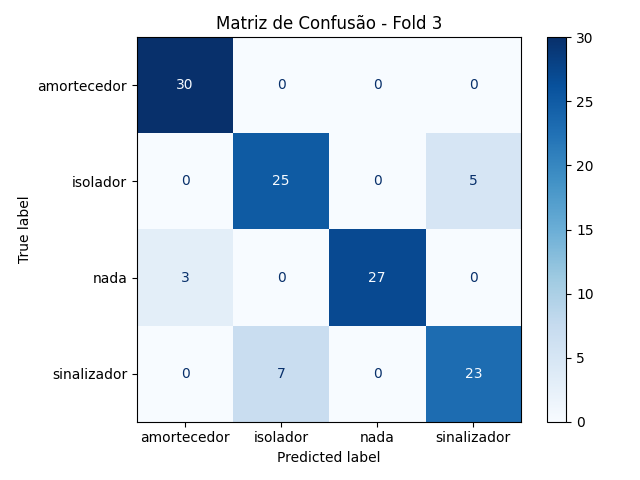
\includegraphics[width=0.7\textwidth]{figuras/Resultados/real_principal_Teste5_nn.png}
\label{fig:matriz_confusao_nn_dobra3}
\fonte{}
\end{figure}


\paragraph{Floresta Aleatória}

\begin{table}[H]
\caption{Desempenho da Floresta Aleatória com features combinadas (real).}
\centering
\begin{tabular}{ccccc}
\hline
\textbf{Dobra} & \textbf{Época Final} & \textbf{Perda Final} & \textbf{Acurácia (\%)} & \textbf{Tempo de Validação (s)}  \\
\hline
1 & - & - & 99.17 & 0.006221 \\
2 & - & - & 100.0 & 0.005471 \\
3 & - & - & 100.0 & 0.005714 \\
4 & - & - & 100.0 & 0.005598 \\
5 & - & - & 100.0 & 0.005813 \\
\hline
\multicolumn{3}{c}{Média} & 99.67 & 0.005763 \\
\hline
\end{tabular}
\fonte{}
\label{tab:resultados_rf_lidar_real}
\end{table}



\section{Resultados com os robôs secundários}

Nesta seção são apresentados os resultados obtidos com os dados provenientes do robôs secundários, utilizados em ambiente simulado. Para ambas topologias analisadas, foi aplicada a validação usando os dados da topologia principal para treinamento e os dados das topologias secundárias para validação, conforme descrito anteriormente. Os resultados estão organizados em subseções separadas, de modo a permitir uma análise clara do desempenho dos modelos em cada tipo de \textit{dataset}. Cada conjunto de dados — imagens brutas, leituras do \textit{LiDAR}, \textit{features} extraídas e combinação de \textit{features} — é avaliado individualmente. As métricas consideradas incluem acurácia média, tempo de validação, perda final e número de épocas, além da matriz de confusão quando relevante. A distinção entre as topologias permite também avaliar a consistência do sensor multimodal frente à variação entre os ambientes.

\subsection{Dados do primeiro robô}

Nesta subseção são apresentados os resultados obtidos a partir dos dados simulados gerados pela primeira topologia secundária em conjunto com os dados do robô principal usados para treinamento.

\subsubsection{Imagens brutas}

Esta subseção apresenta os resultados obtidos com as imagens de profundidade brutas
capturadas pelo primeiro robô das topologias secundárias em ambiente simulado com o modelo treinado pelos dados do robô principal.

\begin{table}[H]
\caption{Desempenho da SqueezeNet com imagens brutas (robô 1 das topologias secundárias).}
\centering
\begin{tabular}{ccccc}
\hline
\textbf{Época Final} & \textbf{Perda Final} & \textbf{Acurácia (\%)} & \textbf{Tempo de Validação (s)}  \\
\hline
3 & 0.00025 & 97.67 & 3.371939 \\
\hline
\end{tabular}
\fonte{}
\label{tab:resultados_nn_topo_secundarias}
\end{table}

\begin{figure}[H]
\centering
\caption{Matriz de confusão do modelo SqueezeNet utilizando imagens brutas (primeiro robô das topologias secundárias).}
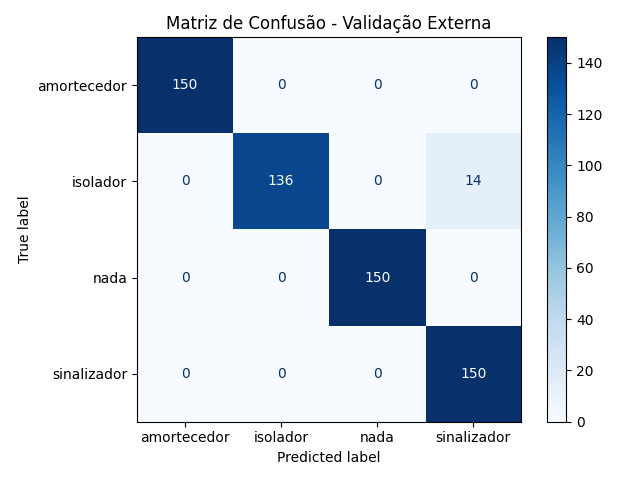
\includegraphics[width=0.7\textwidth]{figuras/Resultados/multi_primeiro_Teste1.png}
\label{fig:mc_squeezenet_imgbrutas_robo1_sim_t1}
\fonte{}
\end{figure}

\subsubsection{Dados brutos do LiDAR}

Esta subseção apresenta os resultados obtidos com os dados brutos do LiDAR capturadas pelo primeiro robô das topologias secundárias em ambiente simulado com o modelo treinado pelos dados do robô principal.

\begin{table}[H]
\caption{Comparativo de desempenho entre diferentes modelos.}
\centering
\begin{tabular}{ccccc}
\hline
\textbf{Modelo} & \textbf{Época Final} & \textbf{Perda Final} & \textbf{Acurácia (\%)} & \textbf{Tempo de Validação (s)}  \\
\hline
kNN      & - & - & 47.83 & 0.01927 \\
Árvore   & - & - & 46.00 & 0.000213 \\ 
Naive    & - & - & 25.00 & 0.000745 \\ 
Rede     & - & - & 25.00 & 0.000745 \\
Floresta & - & - & 46.67 & 0.007682 \\
\hline
\multicolumn{3}{c}{Média} & 38.10 & 0.056262 \\
\hline
\end{tabular}
\fonte{}
\label{tab:comparativo_modelos_atualizado}
\end{table}

\begin{figure}[H]
\centering
\caption{Matriz de confusão para o k-Vizinhos mais próximos com dados brutos do LiDAR (primeiro robô das topologias secundárias).}
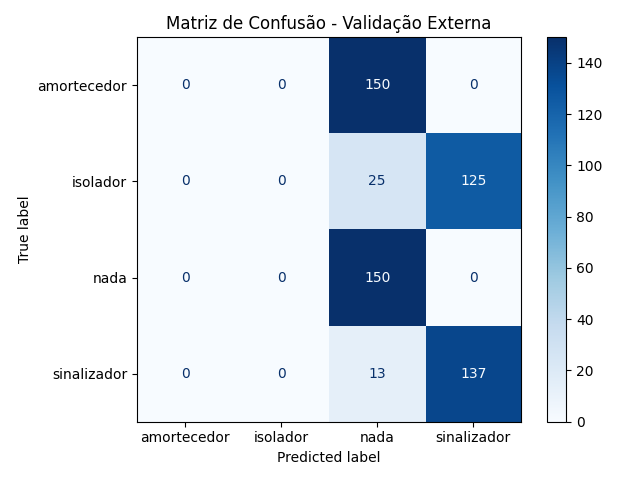
\includegraphics[width=0.7\textwidth]{figuras/Resultados/multi_primeiro_Teste2_knn.png}
\label{fig:mc_lidar_knn_robo1_t2}
\fonte{}
\end{figure}

\begin{figure}[H]
\centering
\caption{Matriz de confusão para a Árvore de Decisão com dados brutos do LiDAR (primeiro robô das topologias secundárias).}
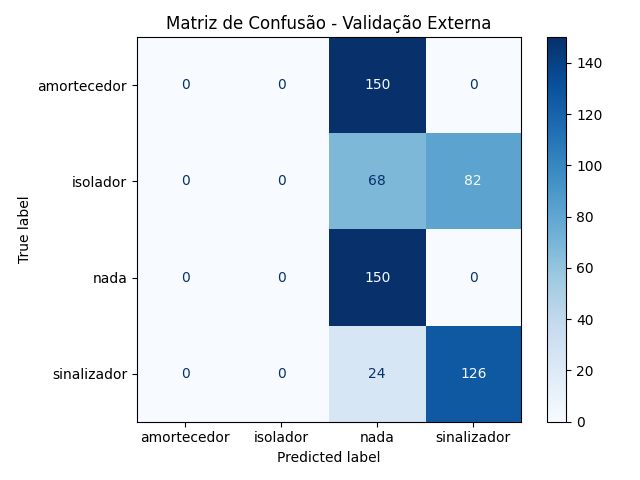
\includegraphics[width=0.7\textwidth]{figuras/Resultados/multi_primeiro_Teste2_tree.png}
\label{fig:mc_lidar_tree_robo1_t2}
\fonte{}
\end{figure}

\begin{figure}[H]
\centering
\caption{Matriz de confusão para o Naive Bayes com dados brutos do LiDAR (primeiro robô das topologias secundárias).}
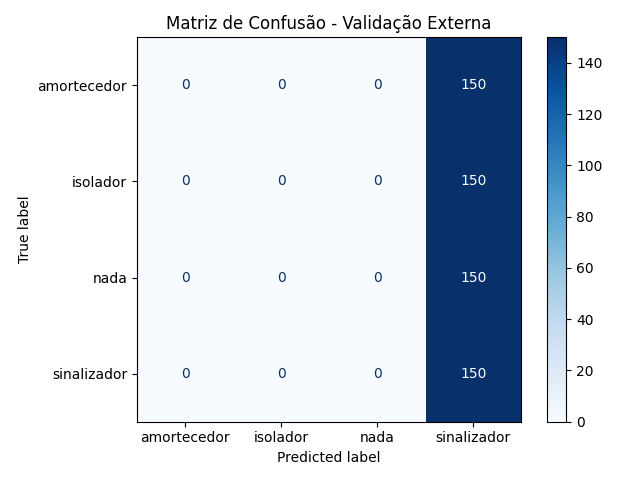
\includegraphics[width=0.7\textwidth]{figuras/Resultados/multi_primeiro_Teste2_naive.png}
\label{fig:mc_lidar_naive_robo1_t2}
\fonte{}
\end{figure}

\begin{figure}[H]
\centering
\caption{Matriz de confusão para a Rede Neural com dados brutos do LiDAR (primeiro robô das topologias secundárias).}
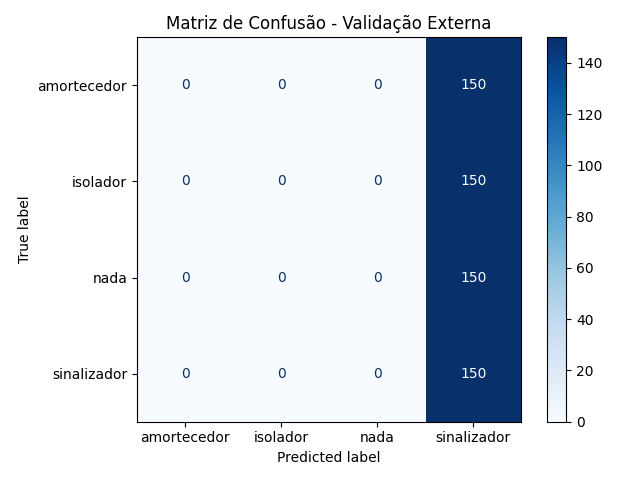
\includegraphics[width=0.7\textwidth]{figuras/Resultados/multi_primeiro_Teste2_nn.png}
\label{fig:mc_lidar_nn_robo1_t2}
\fonte{}
\end{figure}

\begin{figure}[H]
\centering
\caption{Matriz de confusão para a Floresta Aleatória com dados brutos do LiDAR (primeiro robô das topologias secundárias).}
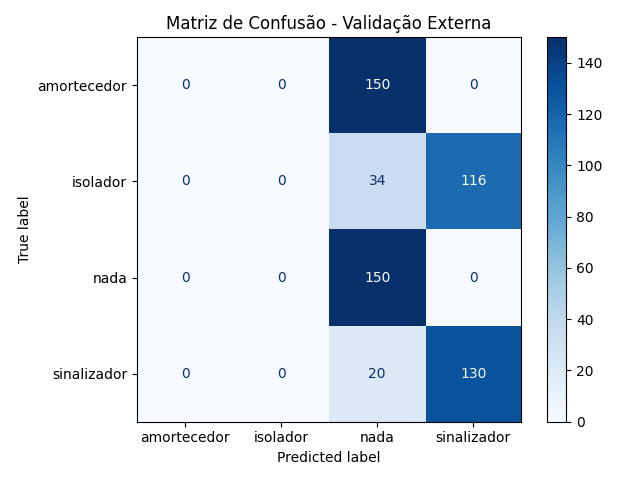
\includegraphics[width=0.7\textwidth]{figuras/Resultados/multi_primeiro_Teste2_rf.png}
\label{fig:mc_lidar_rf_robo1_t2}
\fonte{}
\end{figure}

\subsubsection{Features extraídas das imagens}

Esta subseção apresenta os resultados obtidos a partir de atributos derivados das imagens  capturadas pelo primeiro robô das topologias secundárias em ambiente simulado com o modelo treinado pelos dados do robô principal. As imagens foram processadas para extrair informações relevantes (\textit{features}) que pudessem melhorar a capacidade dos modelos de aprendizado de máquina na identificação das classes de objetos.

\begin{table}[H]
\caption{Desempenho dos modelos com features extraídas das imagens (primeiro robô das topologias secundárias).}
\centering
\begin{tabular}{ccccc}
\hline
\textbf{Modelo} & \textbf{Época Final} & \textbf{Perda Final} & \textbf{Acurácia (\%)} & \textbf{Tempo de Validação (s)}  \\
\hline
kNN      & - & - & 70.33 & 0.012015 \\
Árvore   & - & - & 69.67 & 0.000170 \\
Naive    & - & - & 69.83 & 0.000264 \\
Rede     & 43 & 0.000551 & 75.00 & 0.015986 \\
Floresta & - & - & 69.67 & 0.007539 \\
\hline
\multicolumn{3}{c}{Média} & 70.90 & 0.007195 \\
\hline
\end{tabular}
\fonte{}
\label{tab:modelos_feat_imagens_robo1}
\end{table}


\begin{figure}[H]
\centering
\caption{Matriz de confusão para o k-Vizinhos mais próximos com features extraídas das imagens (primeiro robô das topologias secundárias).}
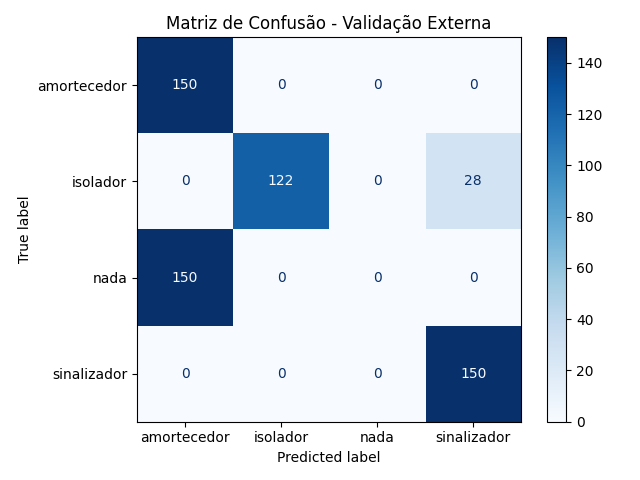
\includegraphics[width=0.7\textwidth]{figuras/Resultados/multi_primeiro_Teste3_knn.png}
\label{fig:mc_featimg_knn_robo1_t3}
\fonte{}
\end{figure}

\begin{figure}[H]
\centering
\caption{Matriz de confusão para a Árvore de Decisão com features extraídas das imagens (primeiro robô das topologias secundárias).}
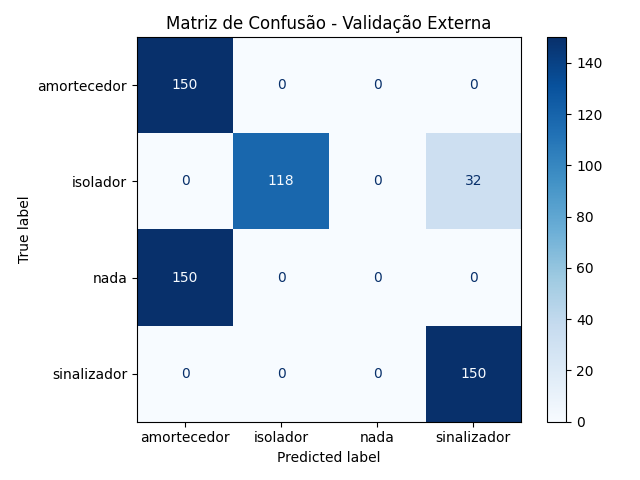
\includegraphics[width=0.7\textwidth]{figuras/Resultados/multi_primeiro_Teste3_tree.png}
\label{fig:mc_featimg_tree_robo1_t3}
\fonte{}
\end{figure}

\begin{figure}[H]
\centering
\caption{Matriz de confusão para o Naive Bayes com features extraídas das imagens (primeiro robô das topologias secundárias).}
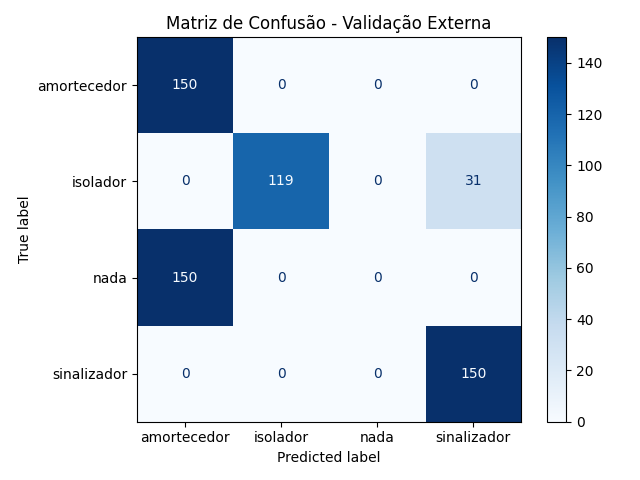
\includegraphics[width=0.7\textwidth]{figuras/Resultados/multi_primeiro_Teste3_naive.png}
\label{fig:mc_featimg_naive_robo1_t3}
\fonte{}
\end{figure}

\begin{figure}[H]
\centering
\caption{Matriz de confusão para a Rede Neural com features extraídas das imagens (primeiro robô das topologias secundárias).}
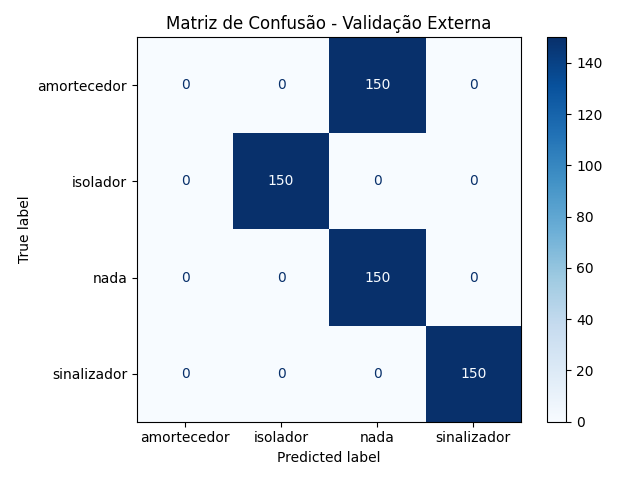
\includegraphics[width=0.7\textwidth]{figuras/Resultados/multi_primeiro_Teste3_nn.png}
\label{fig:mc_featimg_nn_robo1_t3}
\fonte{}
\end{figure}

\begin{figure}[H]
\centering
\caption{Matriz de confusão para a Floresta Aleatória com features extraídas das imagens (primeiro robô das topologias secundárias).}
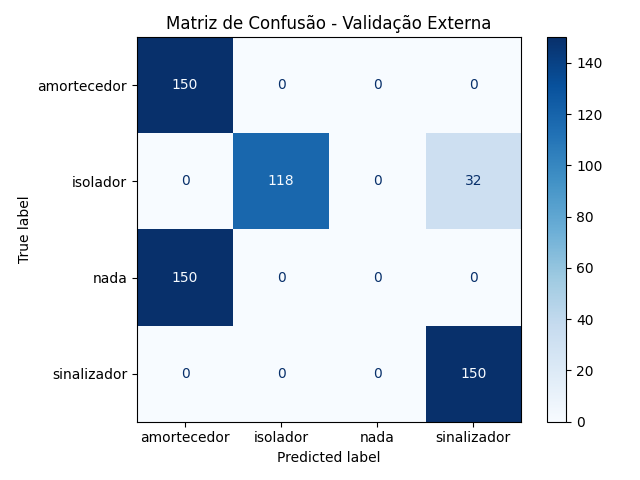
\includegraphics[width=0.7\textwidth]{figuras/Resultados/multi_primeiro_Teste3_rf.png}
\label{fig:mc_featimg_rf_robo1_t3}
\fonte{}
\end{figure}

\subsubsection{Features extraídas do LiDAR}

Esta subseção apresenta os resultados obtidos a partir de atributos derivados dos dados de distância do sensor \textit{LiDAR}, capturadas pelo primeiro robô das topologias secundárias em ambiente simulado com o modelo treinado pelos dados do robô principal. As imagens foram processadas para extrair informações relevantes (\textit{features}) que pudessem melhorar a capacidade dos modelos de aprendizado de máquina na identificação das classes de objetos.

\begin{table}[H]
\caption{Desempenho dos modelos com features extraídas do LiDAR (primeiro robô das topologias secundárias).}
\centering
\begin{tabular}{ccccc}
\hline
\textbf{Modelo} & \textbf{Época Final} & \textbf{Perda Final} & \textbf{Acurácia (\%)} & \textbf{Tempo de Validação (s)}  \\
\hline
kNN      & - & - & 79.83 & 0.012294 \\
Árvore   & - & - & 79.00 & 0.000156 \\
Naive    & - & - & 63.00 & 0.000232 \\
Rede     & 200 & 0.205509 & 69.17 & 0.015490 \\
Floresta & - & - & 80.33 & 0.008353 \\
\hline
\multicolumn{3}{c}{Média} & 74.27 & 0.007305 \\
\hline
\end{tabular}
\fonte{}
\label{tab:modelos_feat_lidar_robo1}
\end{table}

\begin{figure}[H]
\centering
\caption{Matriz de confusão para o k-Vizinhos mais próximos com features extraídas do LiDAR (primeiro robô das topologias secundárias).}
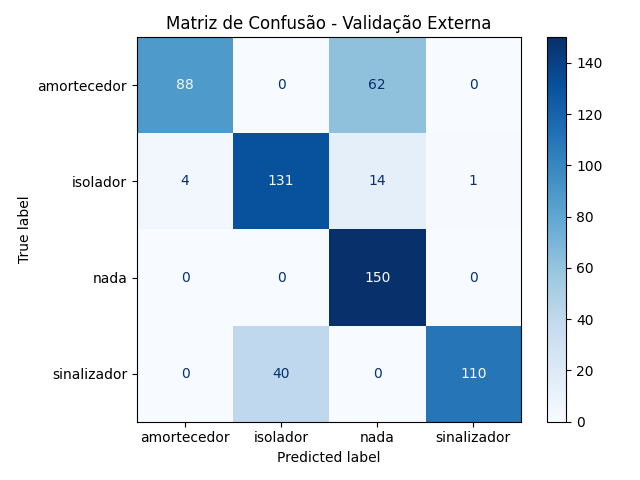
\includegraphics[width=0.7\textwidth]{figuras/Resultados/multi_primeiro_Teste4_knn.png}
\label{fig:mc_featlidar_knn_robo1_t4}
\fonte{}
\end{figure}

\begin{figure}[H]
\centering
\caption{Matriz de confusão para a Árvore de Decisão com features extraídas do LiDAR (primeiro robô das topologias secundárias).}
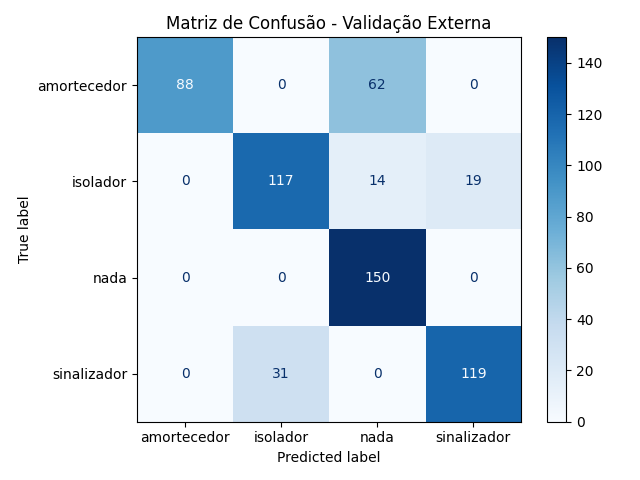
\includegraphics[width=0.7\textwidth]{figuras/Resultados/multi_primeiro_Teste4_tree.png}
\label{fig:mc_featlidar_tree_robo1_t4}
\fonte{}
\end{figure}

\begin{figure}[H]
\centering
\caption{Matriz de confusão para o Naive Bayes com features extraídas do LiDAR (primeiro robô das topologias secundárias).}
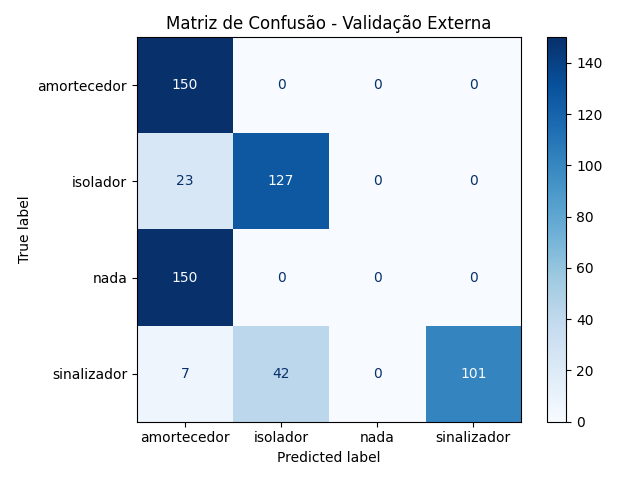
\includegraphics[width=0.7\textwidth]{figuras/Resultados/multi_primeiro_Teste4_naive.png}
\label{fig:mc_featlidar_naive_robo1_t4}
\fonte{}
\end{figure}

\begin{figure}[H]
\centering
\caption{Matriz de confusão para a Rede Neural com features extraídas do LiDAR (primeiro robô das topologias secundárias).}
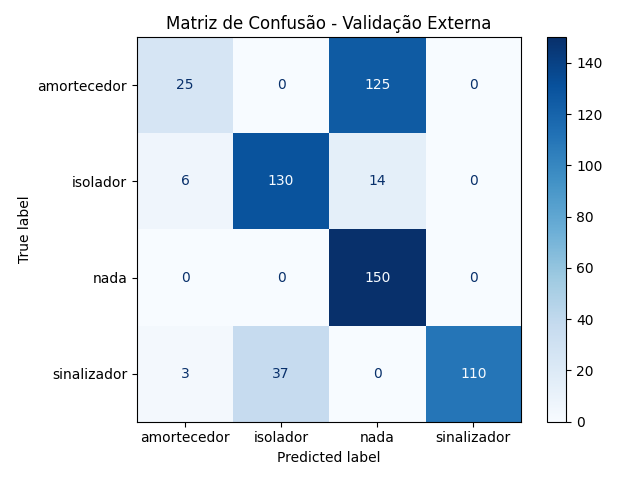
\includegraphics[width=0.7\textwidth]{figuras/Resultados/multi_primeiro_Teste4_nn.png}
\label{fig:mc_featlidar_nn_robo1_t4}
\fonte{}
\end{figure}

\begin{figure}[H]
\centering
\caption{Matriz de confusão para a Floresta Aleatória com features extraídas do LiDAR (primeiro robô das topologias secundárias).}
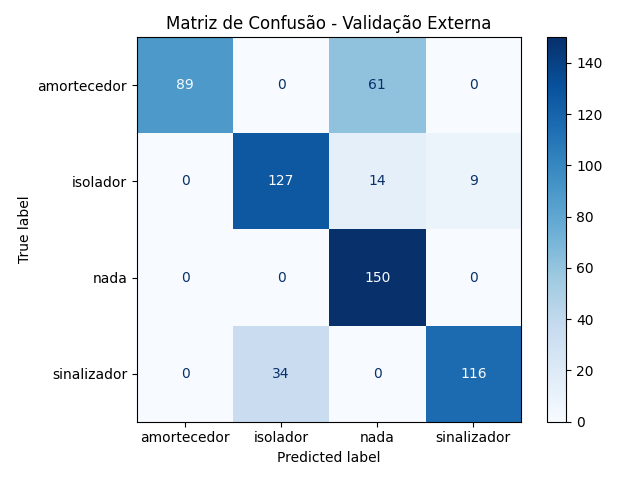
\includegraphics[width=0.7\textwidth]{figuras/Resultados/multi_primeiro_Teste4_rf.png}
\label{fig:mc_featlidar_rf_robo1_t4}
\fonte{}
\end{figure}

\subsubsection{Features combinadas}

Esta subseção apresenta os resultados obtidos a partir da combinação das \textit{features}
extraídas das imagens e dos dados do sensor \textit{LiDAR}, capturadas pelo primeiro robô das topologias secundárias em ambiente simulado com o modelo treinado pelos dados do robô principal.

\begin{table}[H]
\caption{Desempenho dos modelos com features combinadas (primeiro robô das topologias secundárias).}
\centering
\begin{tabular}{ccccc}
\hline
\textbf{Modelo} & \textbf{Época Final} & \textbf{Perda Final} & \textbf{Acurácia (\%)} & \textbf{Tempo de Validação (s)}  \\
\hline
kNN      & - & - & 70.33 & 0.011850 \\
Árvore   & - & - & 69.67 & 0.000151 \\
Naive    & - & - & 69.83 & 0.000245 \\
Rede     & 61 & 0.000034 & 100.00 & 0.016043 \\
Floresta & - & - & 70.33 & 0.007828 \\
\hline
\multicolumn{3}{c}{Média} & 76.03 & 0.007223 \\
\hline
\end{tabular}
\fonte{}
\label{tab:modelos_feat_combinadas_robo1}
\end{table}

\begin{figure}[H]
\centering
\caption{Matriz de confusão para o k-Vizinhos mais próximos com features combinadas (primeiro robô das topologias secundárias).}
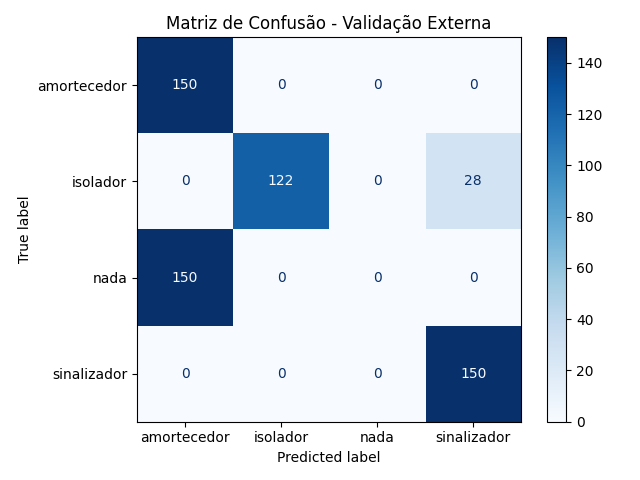
\includegraphics[width=0.7\textwidth]{figuras/Resultados/multi_primeiro_Teste5_knn.png}
\label{fig:mc_featcomb_knn_robo1_t5}
\fonte{}
\end{figure}

\begin{figure}[H]
\centering
\caption{Matriz de confusão para a Árvore de Decisão com features combinadas (primeiro robô das topologias secundárias).}
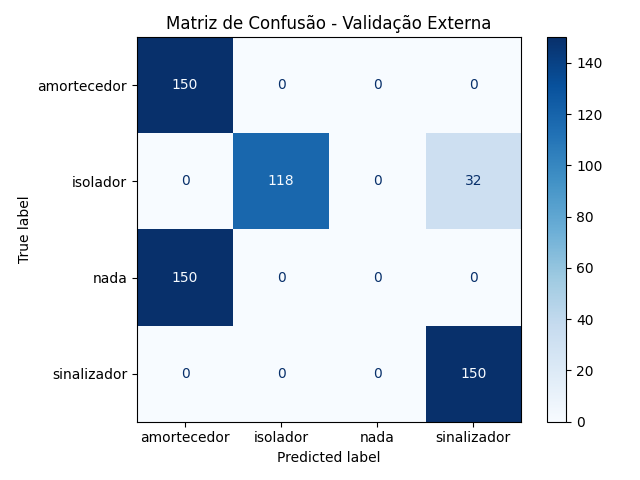
\includegraphics[width=0.7\textwidth]{figuras/Resultados/multi_primeiro_Teste5_tree.png}
\label{fig:mc_featcomb_tree_robo1_t5}
\fonte{}
\end{figure}

\begin{figure}[H]
\centering
\caption{Matriz de confusão para o Naive Bayes com features combinadas (primeiro robô das topologias secundárias).}
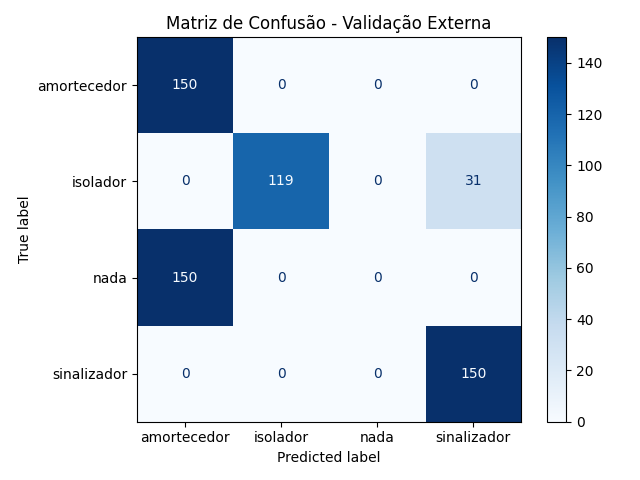
\includegraphics[width=0.7\textwidth]{figuras/Resultados/multi_primeiro_Teste5_naive.png}
\label{fig:mc_featcomb_naive_robo1_t5}
\fonte{}
\end{figure}

\begin{figure}[H]
\centering
\caption{Matriz de confusão para a Floresta Aleatória com features combinadas (primeiro robô das topologias secundárias).}
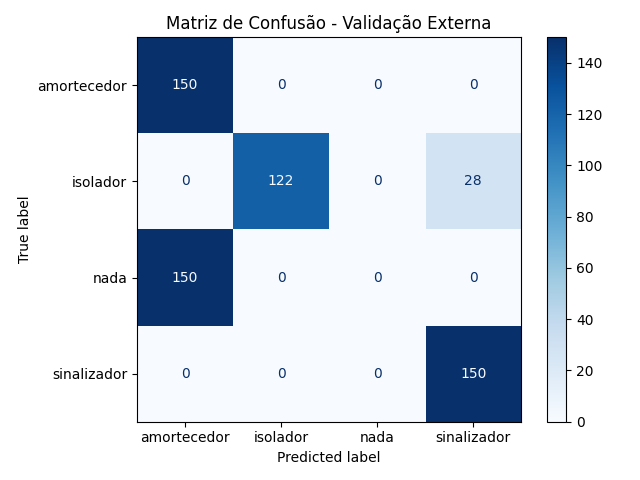
\includegraphics[width=0.7\textwidth]{figuras/Resultados/multi_primeiro_Teste5_rf.png}
\label{fig:mc_featcomb_rf_robo1_t5}
\fonte{}
\end{figure}

\subsection{Dados do segundo robô}

Nesta subseção são apresentados os resultados obtidos a partir dos dados simulados gerados pela segunda topologia secundária em conjunto com os dados do robô principal usados para treinamento. Os resultados serão resumidos nas médias obtidas.

\subsubsection{Imagens brutas}

Esta subseção apresenta os resultados obtidos com as imagens de profundidade brutas
capturadas pelo segundo robô das topologias secundárias em ambiente simulado com o modelo treinado pelos dados do robô principal.


\begin{table}[H]
\caption{Desempenho da SqueezeNet com imagens brutas (robô 1 das topologias secundárias).}
\centering
\begin{tabular}{ccccc}
\hline
\textbf{Época Final} & \textbf{Perda Final} & \textbf{Acurácia (\%)} & \textbf{Tempo de Validação (s)}  \\
\hline
5 & 0.000236 & 97.67 & 3.340613 \\
\hline
\end{tabular}
\fonte{}
\label{tab:resultados_nn2_topo_secundarias}
\end{table}

\subsubsection{Dados brutos do LiDAR}

Esta subseção apresenta os resultados obtidos com os dados brutos do LiDAR capturadas pelo segundo robô das topologias secundárias em ambiente simulado com o modelo treinado pelos dados do robô principal.

\begin{table}[H]
\caption{Desempenho dos modelos com dados brutos do LiDAR (segundo robô das topologias secundárias).}
\centering
\begin{tabular}{ccccc}
\hline
\textbf{Modelo} & \textbf{Época Final} & \textbf{Perda Final} & \textbf{Acurácia (\%)} & \textbf{Tempo de Validação (s)}  \\
\hline
kNN      & - & - & 78.00 & 0.019251 \\
Árvore   & - & - & 52.67 & 0.000230 \\
Naive    & - & - & 36.50 & 0.000785 \\
Rede     & 200 & 0.032724 & 76.33 & 0.015708 \\
Floresta & - & - & 77.50 & 0.007995 \\
\hline
\multicolumn{3}{c}{Média} & 64.20 & 0.043447 \\
\hline
\end{tabular}
\fonte{}
\label{tab:modelos_lidar_bruto_robo2}
\end{table}

% Figuras para a subseção "Dados brutos do LiDAR" (Segundo Robô)
% Contexto: segundo robô das topologias secundárias. Nomes dos arquivos indicam Teste2.

\begin{figure}[H]
\centering
\caption{Matriz de confusão para o k-Vizinhos mais próximos com dados brutos do LiDAR (segundo robô das topologias secundárias).}
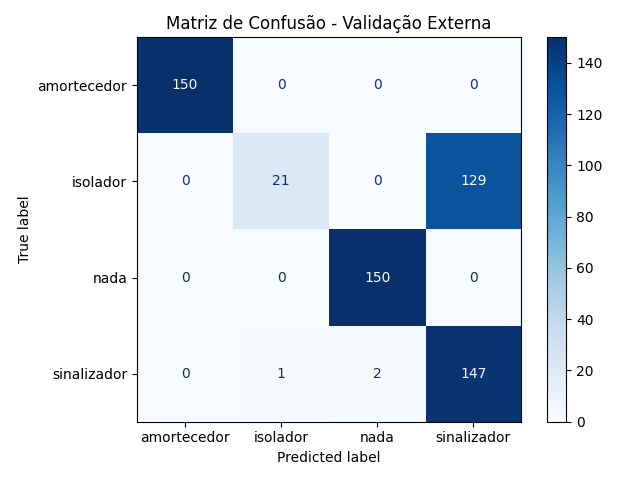
\includegraphics[width=0.7\textwidth]{figuras/Resultados/multi_segundo_Teste2_knn.png}
\label{fig:mc_lidar_knn_robo2_t2}
\fonte{}
\end{figure}

\begin{figure}[H]
\centering
\caption{Matriz de confusão para a Árvore de Decisão com dados brutos do LiDAR (segundo robô das topologias secundárias).}
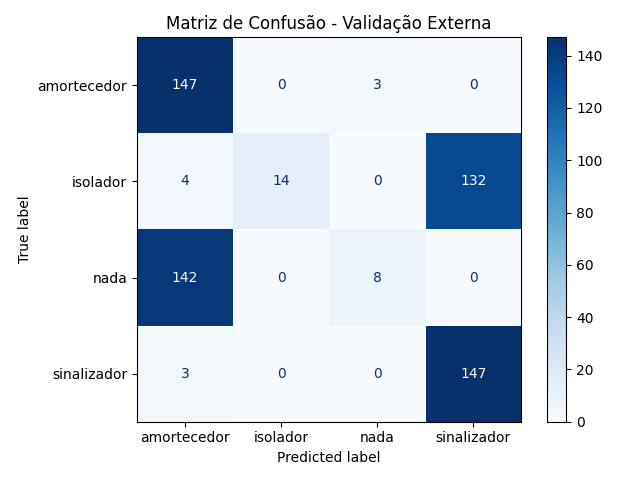
\includegraphics[width=0.7\textwidth]{figuras/Resultados/multi_segundo_Teste2_tree.png}
\label{fig:mc_lidar_tree_robo2_t2}
\fonte{}
\end{figure}

\begin{figure}[H]
\centering
\caption{Matriz de confusão para o Naive Bayes com dados brutos do LiDAR (segundo robô das topologias secundárias).}
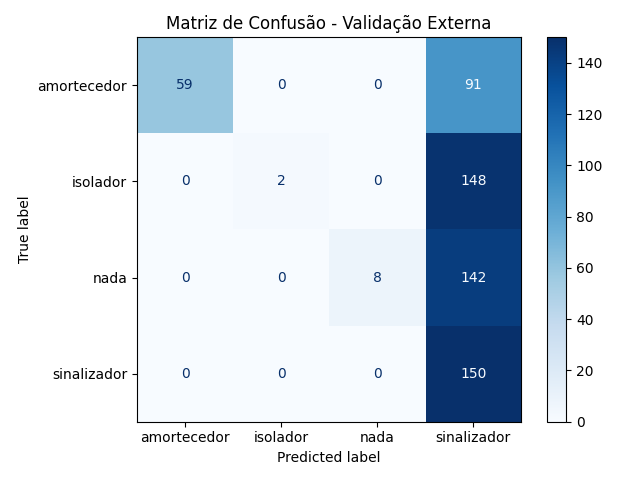
\includegraphics[width=0.7\textwidth]{figuras/Resultados/multi_segundo_Teste2_naive.png}
\label{fig:mc_lidar_naive_robo2_t2}
\fonte{}
\end{figure}

\begin{figure}[H]
\centering
\caption{Matriz de confusão para a Rede Neural com dados brutos do LiDAR (segundo robô das topologias secundárias).}
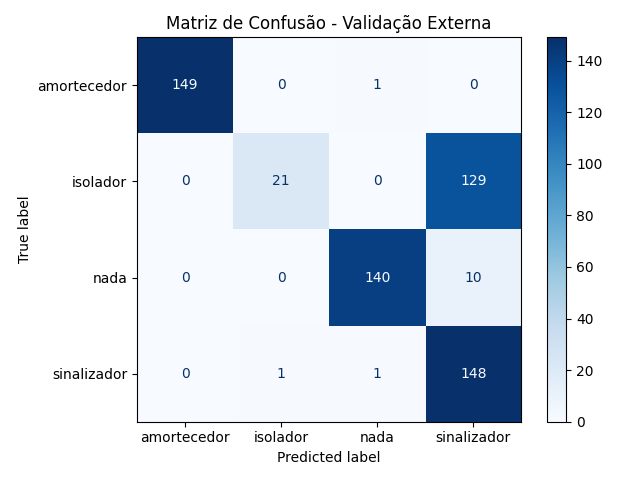
\includegraphics[width=0.7\textwidth]{figuras/Resultados/multi_segundo_Teste2_nn.png}
\label{fig:mc_lidar_nn_robo2_t2}
\fonte{}
\end{figure}

\begin{figure}[H]
\centering
\caption{Matriz de confusão para a Floresta Aleatória com dados brutos do LiDAR (segundo robô das topologias secundárias).}
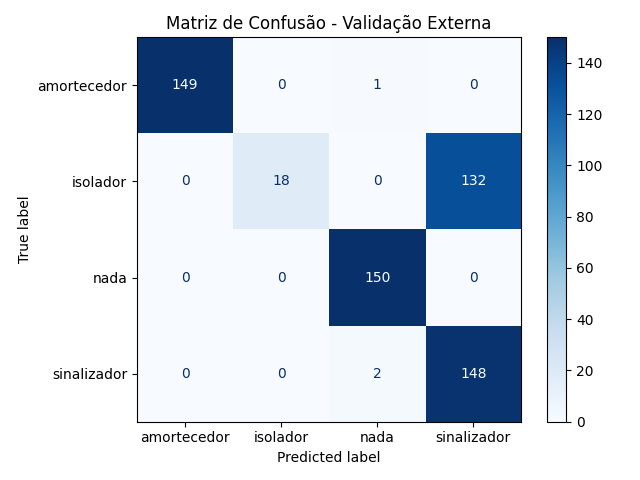
\includegraphics[width=0.7\textwidth]{figuras/Resultados/multi_segundo_Teste2_rf.png}
\label{fig:mc_lidar_rf_robo2_t2}
\fonte{}
\end{figure}

\subsubsection{Features extraídas das imagens}

Esta subseção apresenta os resultados obtidos a partir de atributos derivados das imagens capturadas pelo segundo robô das topologias secundárias em ambiente simulado com o modelo treinado pelos dados do robô principal. As imagens foram processadas para extrair informações relevantes (\textit{features}) que pudessem melhorar a capacidade dos modelos de aprendizado de máquina na identificação das classes de objetos.

\begin{table}[H]
\caption{Desempenho dos modelos com features extraídas das imagens (segundo robô das topologias secundárias).}
\centering
\begin{tabular}{ccccc}
\hline
\textbf{Modelo} & \textbf{Época Final} & \textbf{Perda Final} & \textbf{Acurácia (\%)} & \textbf{Tempo de Validação (s)}  \\
\hline
kNN      & - & - & 86.67 & 0.011986 \\
Árvore   & - & - & 61.17 & 0.000149 \\
Naive    & - & - & 47.33 & 0.000305 \\
Rede     & 60 & 0.000764 & 88.50 & 0.017994 \\
Floresta & - & - & 64.83 & 0.008024 \\
\hline
\multicolumn{3}{c}{Média} & 69.70 & 0.007692 \\
\hline
\end{tabular}
\fonte{}
\label{tab:modelos_featimg_robo2}
\end{table}

% Figuras para a subseção "Features extraídas das imagens" (Segundo Robô)
% Contexto: segundo robô das topologias secundárias. Nomes dos arquivos indicam Teste3.

\begin{figure}[H]
\centering
\caption{Matriz de confusão para o k-Vizinhos mais próximos com features extraídas das imagens (segundo robô das topologias secundárias).}
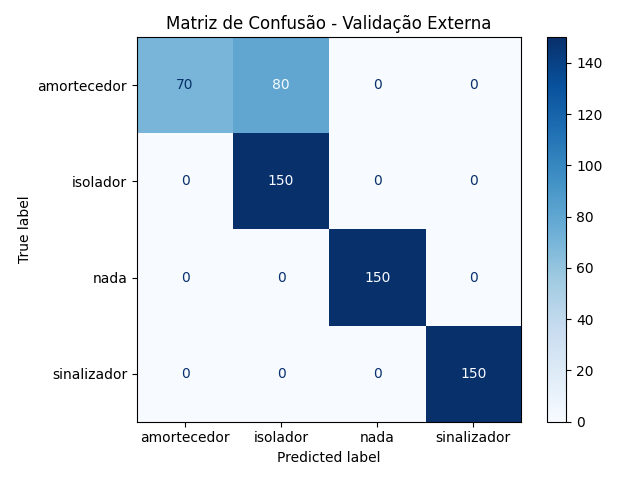
\includegraphics[width=0.7\textwidth]{figuras/Resultados/multi_segundo_Teste3_knn.png}
\label{fig:mc_featimg_knn_robo2_t3}
\fonte{}
\end{figure}

\begin{figure}[H]
\centering
\caption{Matriz de confusão para a Árvore de Decisão com features extraídas das imagens (segundo robô das topologias secundárias).}
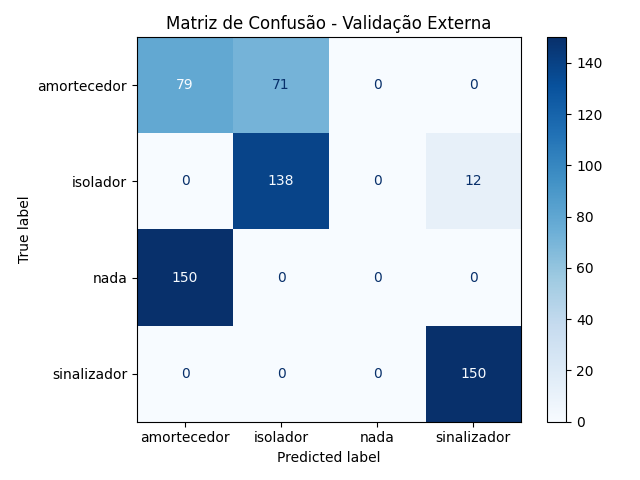
\includegraphics[width=0.7\textwidth]{figuras/Resultados/multi_segundo_Teste3_tree.png}
\label{fig:mc_featimg_tree_robo2_t3}
\fonte{}
\end{figure}

\begin{figure}[H]
\centering
\caption{Matriz de confusão para o Naive Bayes com features extraídas das imagens (segundo robô das topologias secundárias).}
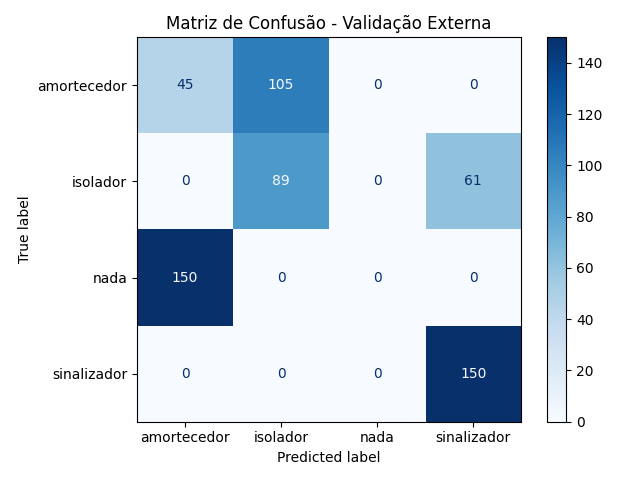
\includegraphics[width=0.7\textwidth]{figuras/Resultados/multi_segundo_Teste3_naive.png}
\label{fig:mc_featimg_naive_robo2_t3}
\fonte{}
\end{figure}

\begin{figure}[H]
\centering
\caption{Matriz de confusão para a Rede Neural com features extraídas das imagens (segundo robô das topologias secundárias).}
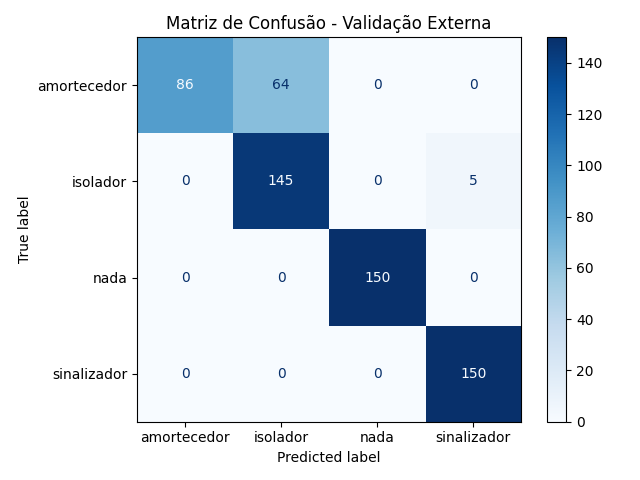
\includegraphics[width=0.7\textwidth]{figuras/Resultados/multi_segundo_Teste3_nn.png}
\label{fig:mc_featimg_nn_robo2_t3}
\fonte{}
\end{figure}

\begin{figure}[H]
\centering
\caption{Matriz de confusão para a Floresta Aleatória com features extraídas das imagens (segundo robô das topologias secundárias).}
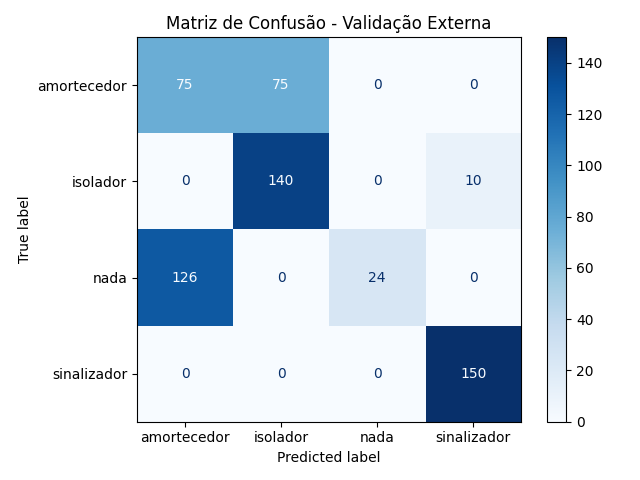
\includegraphics[width=0.7\textwidth]{figuras/Resultados/multi_segundo_Teste3_rf.png}
\label{fig:mc_featimg_rf_robo2_t3}
\fonte{}
\end{figure}

\subsubsection{Features extraídas do LiDAR}

Esta subseção apresenta os resultados obtidos a partir de atributos derivados dos dados de distância do sensor \textit{LiDAR}, capturadas pelo segundo robô das topologias secundárias em ambiente simulado com o modelo treinado pelos dados do robô principal. As imagens foram processadas para extrair informações relevantes (\textit{features}) que pudessem melhorar a capacidade dos modelos de aprendizado de máquina na identificação das classes de objetos.

\begin{table}[H]
\caption{Desempenho dos modelos com features extraídas do LiDAR (segundo robô das topologias secundárias).}
\centering
\begin{tabular}{ccccc}
\hline
\textbf{Modelo} & \textbf{Época Final} & \textbf{Perda Final} & \textbf{Acurácia (\%)} & \textbf{Tempo de Validação (s)}  \\
\hline
kNN      & - & - & 74.33 & 0.013072 \\
Árvore   & - & - & 74.50 & 0.000177 \\
Naive    & - & - & 71.67 & 0.000255 \\
Rede     & 200 & 0.283318 & 93.50 & 0.015820 \\
Floresta & - & - & 80.67 & 0.007872 \\
\hline
\multicolumn{3}{c}{Média} & 78.93 & 0.007439 \\
\hline
\end{tabular}
\fonte{}
\label{tab:modelos_featlidar_robo2}
\end{table}

\begin{figure}[H]
\centering
\caption{Matriz de confusão para o k-Vizinhos mais próximos com features extraídas do LiDAR (segundo robô das topologias secundárias).}
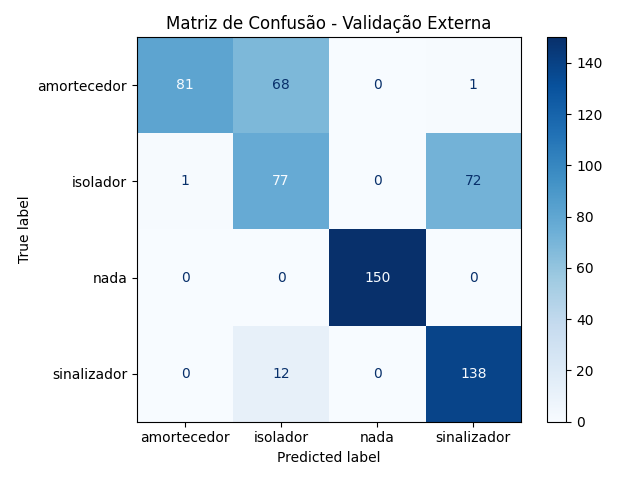
\includegraphics[width=0.7\textwidth]{figuras/Resultados/multi_segundo_Teste4_knn.png}
\label{fig:mc_featlidar_knn_robo2_t4}
\fonte{}
\end{figure}

\begin{figure}[H]
\centering
\caption{Matriz de confusão para a Árvore de Decisão com features extraídas do LiDAR (segundo robô das topologias secundárias).}
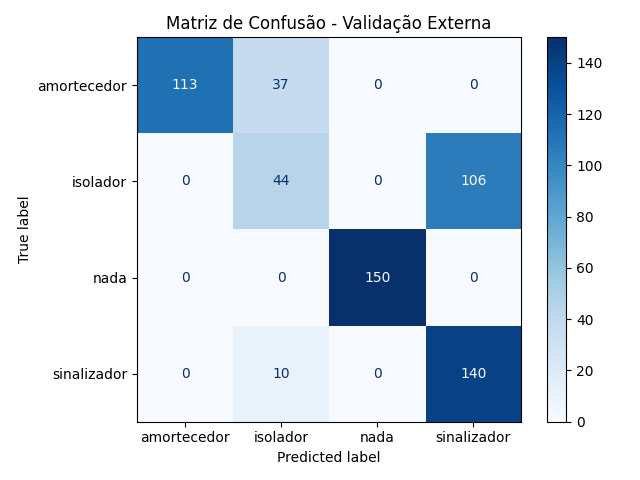
\includegraphics[width=0.7\textwidth]{figuras/Resultados/multi_segundo_Teste4_tree.png}
\label{fig:mc_featlidar_tree_robo2_t4}
\fonte{}
\end{figure}

\begin{figure}[H]
\centering
\caption{Matriz de confusão para o Naive Bayes com features extraídas do LiDAR (segundo robô das topologias secundárias).}
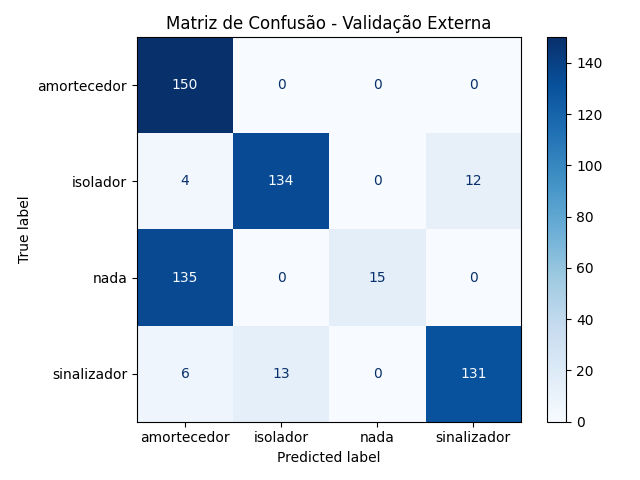
\includegraphics[width=0.7\textwidth]{figuras/Resultados/multi_segundo_Teste4_naive.png}
\label{fig:mc_featlidar_naive_robo2_t4}
\fonte{}
\end{figure}

\begin{figure}[H]
\centering
\caption{Matriz de confusão para a Rede Neural com features extraídas do LiDAR (segundo robô das topologias secundárias).}
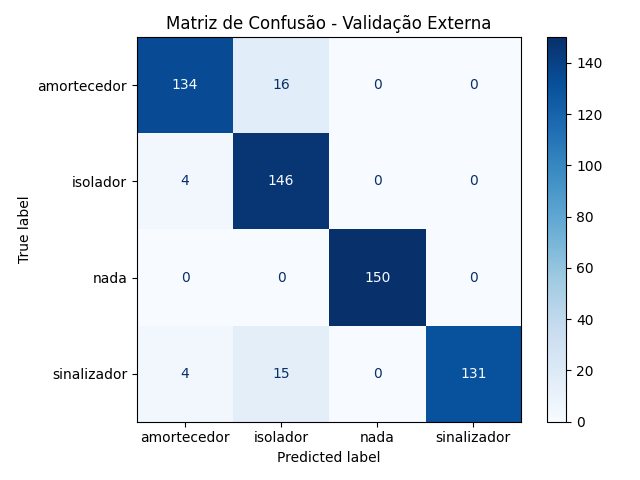
\includegraphics[width=0.7\textwidth]{figuras/Resultados/multi_segundo_Teste4_nn.png}
\label{fig:mc_featlidar_nn_robo2_t4}
\fonte{}
\end{figure}

\begin{figure}[H]
\centering
\caption{Matriz de confusão para a Floresta Aleatória com features extraídas do LiDAR (segundo robô das topologias secundárias).}
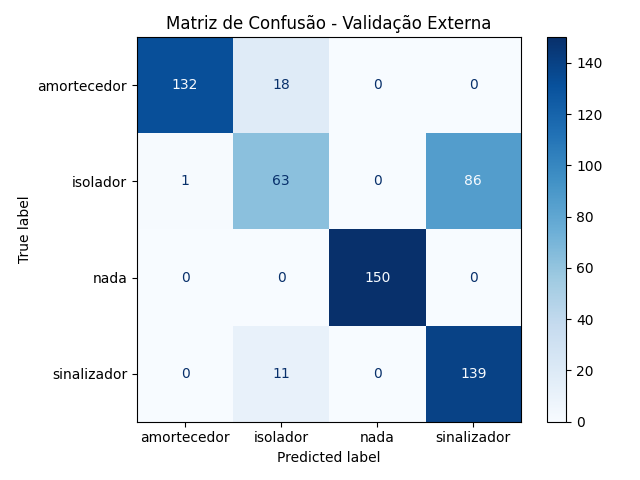
\includegraphics[width=0.7\textwidth]{figuras/Resultados/multi_segundo_Teste4_rf.png}
\label{fig:mc_featlidar_rf_robo2_t4}
\fonte{}
\end{figure}

\subsubsection{Features combinadas}

Esta subseção apresenta os resultados obtidos a partir da combinação das \textit{features}
extraídas das imagens e dos dados do sensor \textit{LiDAR}, capturadas pelo segundo robô das topologias secundárias em ambiente simulado com o modelo treinado pelos dados do robô principal.

\begin{table}[H]
\caption{Desempenho dos modelos com features combinadas (segundo robô das topologias secundárias).}
\centering
\begin{tabular}{ccccc}
\hline
\textbf{Modelo} & \textbf{Época Final} & \textbf{Perda Final} & \textbf{Acurácia (\%)} & \textbf{Tempo de Validação (s)}  \\
\hline
kNN      & - & - & 86.67 & 0.011865 \\
Árvore   & - & - & 84.67 & 0.000149 \\
Naive    & - & - & 49.50 & 0.000358 \\
Rede     & 71 & 0.000686 & 88.50 & 0.015628 \\
Floresta & - & - & 64.83 & 0.006904 \\
\hline
\multicolumn{3}{c}{Média} & 74.83 & 0.006981 \\
\hline
\end{tabular}
\fonte{}
\label{tab:modelos_featcomb_robo2}
\end{table}

\begin{figure}[H]
\centering
\caption{Matriz de confusão para o k-Vizinhos mais próximos com features combinadas (segundo robô das topologias secundárias).}
\includegraphics[width=0.7\textwidth]{figuras/Resultados/multi_segundo_Teste5_knn.png}
\label{fig:mc_featcomb_knn_robo2_t5}
\fonte{}
\end{figure}

\begin{figure}[H]
\centering
\caption{Matriz de confusão para a Árvore de Decisão com features combinadas (segundo robô das topologias secundárias).}
\includegraphics[width=0.7\textwidth]{figuras/Resultados/multi_segundo_Teste5_tree.png}
\label{fig:mc_featcomb_tree_robo2_t5}
\fonte{}
\end{figure}

\begin{figure}[H]
\centering
\caption{Matriz de confusão para o Naive Bayes com features combinadas (segundo robô das topologias secundárias).}
\includegraphics[width=0.7\textwidth]{figuras/Resultados/multi_segundo_Teste5_naive.png}
\label{fig:mc_featcomb_naive_robo2_t5}
\fonte{}
\end{figure}

\begin{figure}[H]
\centering
\caption{Matriz de confusão para a Rede Neural com features combinadas (segundo robô das topologias secundárias).}
\includegraphics[width=0.7\textwidth]{figuras/Resultados/multi_segundo_Teste5_nn.png}
\label{fig:mc_featcomb_nn_robo2_t5}
\fonte{}
\end{figure}

\begin{figure}[H]
\centering
\caption{Matriz de confusão para a Floresta Aleatória com features combinadas (segundo robô das topologias secundárias).}
\includegraphics[width=0.7\textwidth]{figuras/Resultados/multi_segundo_Teste5_rf.png}
\label{fig:mc_featcomb_rf_robo2_t5}
\fonte{}
\end{figure}

%-----------------------------------------------------------%